\chapter{Rings and Ideals}
\label{ch:1}

\begin{exercise}
\label{ex:1.1}
Let $x$ be a nilpotent element of a ring $A$.
Show that $1 + x$ is a unit of $A$.
Deduce that the sum of a nilpotent element and a unit is a unit.
\end{exercise}

\begin{proof}
Choose a positive integer $n$ such that $x^n = 0$.
Then
\begin{align*}
(1 + x) (1 - x + x^2 - \cdots + (-1)^{n-1} x^{n-1})
= 1 + (-1)^{n-1}x^n
= 1
\end{align*}
which shows that $1 + x$ is a unit.
(Alternatively, since the nilradical of $A$ is contained in the Jacobson radical of $A$, $1 + x$ is a unit by Proposition 1.9.)

Next, let $x\in A$ be nilpotent and $u\in A$ a unit.
Then $ux$ is nilpotent, so $1 + ux$ is a unit by the first part.
Therefore
\begin{equation*}
u + x = u^{-1}(1 + ux)
\end{equation*}
is a product of units, so it is a unit.
\end{proof}




\begin{exercise}
\label{ex:1.2}
Let $A$ be a ring and let $A[x]$ be the ring of polynomials in an indeterminate $x$, with coefficients in $A$.
Let $f = a_0 + a_1 x + \cdots + a_n x^n \in A[x]$.
Prove that
\begin{rlist}
\item
\label{ex:1.2.i}
$f$ is a unit in $A[x]$ $\iff$ $a_0$ is a unit in $A$ and $a_1,\ldots,a_n$ are nilpotent.
[If $b_0+b_1 x + \cdots + b_m x^m$ is the inverse of $f$, prove by induction on $r$ that $a_n^{r+1} b_{m-r} = 0$.
Hence show that $a_n$ is nilpotent, and then use Ex. 1.]
\item
\label{ex:1.2.ii}
$f$ is a nilpotent $\iff$ $a_0,a_1,\ldots,a_n$ are nilpotent.
\item
\label{ex:1.2.iii}
$f$ is a zero-divisor $\iff$ there exists $a \neq 0$ in $A$ such that $a f = 0$.
[Choose a polynomial $g = b_0 + b_1 x + \cdots + b_m x^m$ of least degree $m$ such that $f g = 0$.
Then $a_n b_m = 0$, hence $a_n g = 0$ (because $a_n g$ annihilates $f$ and has degree $< m$).
Now show by induction that $a_{n-r} g = 0$ ($0 \leq r \leq n$).]
\item
\label{ex:1.2.iv}
$f$ is said to be \emph{primitive} if $(a_0,a_1,\ldots,a_n)=(1)$.
Prove that if $f,g\in A[x]$, then $fg$ is primitive $\iff$ $f$ and $g$ are primitive.
\end{rlist}
\end{exercise}

\noindent
\ref{ex:1.2.i}
($\Leftarrow$)
If $a_1,\ldots,a_n$ are nilpotent in $A$, then they are also nilpotent in $A[x]$.
Since the nilradical of $A[x]$ is an ideal (Proposition 1.7), $a_1 x + \cdots + a_n x^n$ is nilpotent in $A[x]$.
Moreover, if $a_0$ is unit, then $a_0$ is a unit in $A[x]$, whence
\begin{equation*}
f = a_0 + (a_1 x + \cdots + a_n x^n)
\end{equation*}
is a unit by Exercise \ref{ex:1.1}.

($\Rightarrow$)
Suppose $f$ is a unit in $A[x]$, and let $g \in A[x]$ be its inverse, with constant term $b_0$.
The constant term of the product $f g = 1$ is $a_0 b_0 = 1$, so $a_0$ is a unit in $A$.

Next, let $\mathfrak p$ be a prime ideal of $A$, and let $\overline f$ and $\overline g$ be the reductions of $f$ and $g$ modulo $\mathfrak p$.
Since $(A/\mathfrak p)[x]$ is an integral domain, the equality $\overline f \overline g = 1$ implies
\begin{equation*}
\deg \overline f + \deg \overline g = 0.
\end{equation*}
Therefore $\overline f$ is a constant polynomial in $(A/\mathfrak p)[x]$.
It follows that $a_1,\ldots,a_n \in \mathfrak p$, and since $\mathfrak p$ was arbitrarily chosen, it follows that $a_1,\ldots, a_n$ are contained in the nilradical of $A$ by Proposition 1.8.
\qed

\noindent
\ref{ex:1.2.ii}
($\Leftarrow$)
If $a_0,\ldots,a_n$ are nilpotent in $A$, then they are also nilpotent in $A[x]$.
Since the nilradical of $A[x]$ is an ideal (Proposition 1.7), it follows that $f = a_0 + a_1 x + \cdots + a_n x^n$ is nilpotent in $A[x]$.

($\Rightarrow$)
Suppose $f$ is nilpotent, and let $\mathfrak p$ be a prime ideal of $A$.
The reduction of $f$ modulo $\mathfrak p$ is nilpotent in the integral domain $(A/\mathfrak p)[x]$, whence it is zero modulo $\mathfrak p$.
Therefore $a_0,a_1,\ldots,a_n \in \mathfrak p$, and the arbitrary choice of $\mathfrak p$ implies that $a_0,\ldots,a_n$ are in the nilradical of $A$ by Proposition 1.8.
\qed

\noindent
\ref{ex:1.2.iii}
(This is apparently due to McCoy--cf. \cite[Theorem 2]{McCoyDivisorsOfZero}.)

($\Leftarrow$)
If there exists a nonzero $a \in A$ such that $a f = 0$, then $f$ is a zero-divisor by definition.

($\Rightarrow$)
Suppose $f$ is a zero-divisor, and let $g \in A[x]$ be a polynomial of least degree $m$ such that $g f = 0$.
Write
\begin{equation*}
g = b_0 + b_1 x + \cdots + b_m x^m.
\end{equation*}
The $(m+n)$th coefficient of the product $f g = 0$ is $a_n b_m = 0$, so $a_n g$ has degree less than $m$.
Moreover, since $g f = 0$, we also have $(a_n g) f = 0$, so by the minimality of $m$, it follows that $a_n g = 0$.

Next, suppose $r\in\{0,\ldots,n-1\}$ satisfies
\begin{equation*}
a_n g
= a_{n-1} g
= \cdots
= a_{n-r} g
= 0.
\end{equation*}
Then we have
\begin{align*}
0
= f g
&= a_0 g + a_1 g x + \cdots + a_n g x^n
\\&= a_0 g + a_1 g x + \cdots + a_{n-r-1} g x^{n-r-1}.
\end{align*}
The highest-degree coefficient of the final sum above is $a_{n-r-1} b_m = 0$, so $a_{n-r-1} g$ has degree less than $m$.
Again we have $(a_{n-r-1} g) f = 0$, whence $a_{n-r-1} g = 0$ by the minimality of the degree of $g$.

By induction on $r$, we conclude that $a_{n-r} g = 0$ for $0 \leq r \leq n$.
In particular, $a_j b_m = 0$ for $0\leq j \leq n$, so that $b_m f = 0$.
\qed

\noindent
\ref{ex:1.2.iv}
Let
\begin{equation*}
f = a_0 + a_1 x + \cdots + a_n x^n,
\qquad
g = b_0 + b_1 x + \cdots + b_m x^m
\end{equation*}
be polynomials in $A[x]$, and let
\begin{equation*}
g f = c_0 + c_1 x + \cdots + c_{m+n} x^{m+n}
\end{equation*}
be their product, where
\begin{equation*}
c_k = \sum_{\substack{i+j=k \\ 0\leq i\leq n\\0\leq j\leq m}} a_i b_j.
\end{equation*}
Define the ideals $\mathfrak a = (a_0,\ldots,a_n)$, $\mathfrak b = (b_0,\ldots,b_m)$, and $\mathfrak c = (c_0,\ldots,c_{m+n})$ of $A$.
Clearly $\mathfrak c \subseteq \mathfrak a \cap \mathfrak b$.

($\Rightarrow$)
Suppose $f g$ is primitive, so that $\mathfrak c = (1)$.
Since $\mathfrak c \subseteq \mathfrak a \cap \mathfrak b$, it follows that $\mathfrak a = \mathfrak b = (1)$, so $f$ and $g$ are primitive.

($\Leftarrow$)
Suppose $f g$ is not primitive, so that $\mathfrak c \neq (1)$.
Then by Corollary 1.4, there exists a maximal ideal $\mathfrak m$ of $A$ with $\mathfrak c \subseteq \mathfrak m$.
Let $\overline f$ and $\overline g$ be the reductions of $f$ and $g$ modulo $\mathfrak m$.
Since $(A/\mathfrak m)[x]$ is an integral domain and $\mathfrak m$ contains the coefficients of $f g$, it follows that $\overline f \overline g = 0$, so either $\overline f = 0$ or $\overline g = 0$.
Thus, either the coefficients of $f$ or the coefficients of $g$ are contained in $\mathfrak m$, whence either $\mathfrak a$ or $\mathfrak b$ is not the unit ideal.
Therefore either $f$ is not primitive or $g$ is not primitive.
\qed





\begin{exercise}
\label{ex:1.3}
Generalize the results of Exercise \ref{ex:1.2} to a polynomial ring $A[x_1,\ldots,x_r]$ in several indeterminates.
\end{exercise}




\begin{claim}[Generalization of Exercise \ref{ex:1.2}\ref{ex:1.2.ii}]
\label{claim:1.3.ii}
A polynomial $f\in A[x_1,\ldots,x_r]$ is nilpotent if and only if its coefficients are all nilpotent.
\end{claim}

\begin{proof}
($\Leftarrow$)
Same as the original proof of this direction of Exercise \ref{ex:1.2}\ref{ex:1.2.ii}.

($\Rightarrow$)
We induct on $r$, with the $r=1$ case being handled by Exercise \ref{ex:1.2}\ref{ex:1.2.ii}.
Consider a nilpotent $f \in A[x_1,\ldots,x_r]$, with $r > 1$, and write $f$ as a single-variable polynomial (in the indeterminate $x_r$) with coefficients in $A[x_1,\ldots,x_{r-1}]$:
\begin{equation*}
f = f_0 + f_1 x_r + \cdots + f_n x_r^n,
\end{equation*}
with each $f_i \in A[x_1,\ldots,x_{r-1}]$.
Since $f$ is nilpotent, Exercise \ref{ex:1.2}\ref{ex:1.2.ii} implies that each $f_i$ is nilpotent in $A[x_1,\ldots,x_{r-1}]$.
By induction, we conclude that the coefficients of each $f_i$ are nilpotent, and therefore the coefficients of $f$ are nilpotent.
\end{proof}


\begin{claim}[Generalization of Exercise \ref{ex:1.2}\ref{ex:1.2.i}]
\label{claim:1.3.i}
A polynomial $f\in A[x_1,\ldots,x_r]$ is a unit if and only if its constant term is a unit in $A$ and the rest of the coefficients are nilpotent.
\end{claim}

\begin{proof}
($\Leftarrow$)
Same as the original proof of this direction of Exercise \ref{ex:1.2}\ref{ex:1.2.i}.

($\Rightarrow$)
We induct on $r$, with the $r=1$ case being handled by Exercise \ref{ex:1.2}\ref{ex:1.2.i}.
Consider an invertible $f \in A[x_1,\ldots,x_r]$, with $r > 1$.
Again, write
\begin{equation*}
f = f_0 + f_1 x_r + \cdots + f_n x_r^n,
\end{equation*}
with each $f_i \in A[x_1,\ldots,x_{r-1}]$.
By Exercise \ref{ex:1.2}\ref{ex:1.2.i}, $f_0$ is a unit in $A[x_1,\ldots,x_{r-1}]$ and $f_1,\ldots,f_n$ are nilpotent.
By Claim \ref{claim:1.3.i}, the coefficients of the polynomials $f_1,\ldots,f_n$ are nilpotent.
Moreover, by induction the constant term of $f_0$ is a unit and its other coefficients are nilpotent.
Therefore the constant term of $f$ is a unit, and the remaining coefficients are nilpotent.
\end{proof}


\begin{claim}[Generalization of Exercise \ref{ex:1.2}\ref{ex:1.2.iii}]
\label{claim:1.3.iii}
A polynomial $f\in A[x_1,\ldots,x_r]$ is a zero-divisor if and only if there exists a nonzero $a \in A$ such that $a f = 0$.
\end{claim}

\begin{proof}
($\Leftarrow$)
Nothing to prove.

($\Rightarrow$)
We induct on $r$, with the $r=1$ case being handled by Exercise \ref{ex:1.2}\ref{ex:1.2.iii}.
Suppose $r > 1$ and $f \in A[x_1,\ldots,x_r]$ is a zero-divisor.
As before, write
\begin{equation*}
f = f_0 + f_1 x_r + \cdots + f_n x_r^n,
\end{equation*}
with each $f_i \in A[x_1,\ldots,x_{r-1}]$.
Since $f$ is a zero-divisor in the polynomial ring $A[x_1,\ldots,x_{r-1}][x_r]$, by Exercise \ref{ex:1.2}\ref{ex:1.2.iii} there exists a nonzero $g \in A[x_1,\ldots,x_{r-1}]$ such that $g f = 0$.
In particular, $g f_i = 0$ for all $i$.
Let $d_i$ be the highest power of $x_{r-1}$ occurring in $f_i$, and let
\begin{equation*}
d = \max\{d_0,d_1,\ldots,d_{r-1}\}+1.
\end{equation*}
Then, define
\begin{equation*}
h
= f_0 + f_1 x_{r-1}^d + \cdots + f_n x_{r-1}^{nd},
\end{equation*}
a polynomial in $A[x_1,\ldots,x_{r-1}]$.
Then $g h = 0$, so by induction, there exists a non-zero $a \in A$ such that $a h = 0$.
In particular, $a$ annihilates all the coefficients of $h$, and these, by the construction of $h$, are exactly the coefficients of $f_0,f_1,\ldots,f_n$.
Thus $a f_i = 0$ for each $i$, and hence $a f = 0$.
\end{proof}

\begin{claim}[Generalization of Exercise \ref{ex:1.2}\ref{ex:1.2.iv}]
\label{claim:1.3.iv}
Let $f,g\in A[x_1,\ldots,x_r]$ be given.
Then $f g$ is primitive if and only if $f$ and $g$ are primitive
\end{claim}

\begin{proof}
The same proof as the proof of Exercise \ref{ex:1.2}\ref{ex:1.2.iv} works here if we define $\mathfrak a$, $\mathfrak b$, and $\mathfrak c$ to be the ideals generated by the coefficients of $f$, $g$, and $f g$, respectively.
\end{proof}







\begin{exercise}
\label{ex:1.4}
In the ring $A[x]$, the Jacobson radical is equal to the nilradical.
\end{exercise}

\begin{proof}
Let $\mathfrak R$ and $\mathfrak R$ be the nilradical and Jacobson radical of $A[x]$, respectively.
We necessarily have $\mathfrak N \subseteq \mathfrak R$, so it suffices to prove that $\mathfrak R \subseteq \mathfrak N$.
Let $f \in \mathfrak R$ be given.
By Proposition 1.9, $1 + x f$ is a unit in $A[x]$, so by Exercise \ref{ex:1.2}\ref{ex:1.2.i}, the coefficients of the non-constant terms of $1 + x f$ are nilpotent.
Thus, the coefficients of $x f$, and hence of $f$, are nilpotent, and so $f$ itself is nilpotent by Exercise \ref{ex:1.2}\ref{ex:1.2.ii}, and hence $\mathfrak R \subseteq \mathfrak N$.
\end{proof}





\begin{exercise}
\label{ex:1.5}
Let $A$ be a ring and let $A[[x]]$ be the ring of formal power series $f = \sum_{n=0}^\infty a_n x^n$ with coefficients in $A$.
Show that
\begin{rlist}
\item
\label{ex:1.5.i}
$f$ is a unit in $A[[x]]$ $\iff$ $a_0$ is a unit in $A$.
\item
\label{ex:1.5.ii}
If $f$ is nilpotent, then $a_n$ is nilpotent for all $n\geq 0$.
Is the converse true?
(See Chapter \ref{ch:7}, Exercise \ref{ex:7.2}.)
\item
\label{ex:1.5.iii}
$f$ belongs to the Jacobson radical of $A[[x]]$ $\iff$ $a_0$ belongs to the Jacobson radical of $A$.
\item
\label{ex:1.5.iv}
The contraction of a maximal ideal $\mathfrak m$ of $A[[x]]$ is a maximal ideal of $A$, and $\mathfrak m$ is generated by $\mathfrak m^c$ and $x$.
\item
\label{ex:1.5.v}
Every prime ideal of $A$ is the contraction of a prime ideal of $A[[x]]$.
\end{rlist}
\end{exercise}

\noindent
We will occasionally need to use the following claim.

\begin{claim}
\label{claim:1.5.power series integral domain}
If $A$ is an integral domain, then $A[[x]]$ is an integral domain.
\end{claim}

\begin{proof}
Suppose $A$ is an integral domain, and suppose $f,g\in A[[x]]$ are nonzero.
Write
\begin{equation*}
f = \sum_{n=0}^\infty a_n x^n,
\qquad
g = \sum_{n=0}^\infty b_n x^n,
\qquad
f g = \sum_{n=0}^\infty c_n x^n,
\end{equation*}
where
\begin{equation*}
c_n = \sum_{i + j = n} a_i b_j.
\end{equation*}
Choose the least non-negative integers $i_0$ and $j_0$ such that $a_{i_0} \neq 0$ and $b_{i_0} \neq 0$.
Thus, $a_{i_0} b_{j_0} \neq 0$, and $a_i = b_j = 0$ for $i < i_0$ and $j < j_0$.
If $n = i_0 + j_0$, then we have
\begin{equation*}
c_n = a_{i_0} b_{j_0} + \sum_{\substack{i + j = k \\ i \neq i_0}} a_i b_j.
\end{equation*}
In every summand of the sum above, either $i < i_0$ or $j < j_0$.
Thus, the sum is zero, whence $c_n = a_{i_0} b_{j_0} \neq 0$, and hence $f g \neq 0$.
Therefore, $A[[x]]$ is an integral domain.
\end{proof}

\noindent
\ref{ex:1.5.i}
($\Rightarrow$)
If $f\in A[[x]]$ is a unit with inverse $g\in A[[x]]$, then looking at the constant term of $f g = 1$ shows that $a_0$ is a unit.

($\Leftarrow$)
Suppose $a_0$ is invertible.
We define a sequence $b_0,b_1,b_2,\ldots \in A$ recursively as follows.
Let $b_0 = a_0^{-1}$.
Next, having defined $b_0,\ldots,b_{r-1}$, define
\begin{equation*}
b_r = -a_0^{-1}\sum_{k=1}^r a_k b_{r-k}.
\end{equation*}
Now let $g \in A[[x]]$ be the formal power series $g = \sum_{n=0}^\infty b_n x^n$.
Then the product $f g$ has the power series expansion $f g = \sum_{n=0}^\infty c_n x^n$, where
\begin{equation*}
c_n = \sum_{k=0}^n a_k b_{n-k}.
\end{equation*}
It follows that $c_0 = a_0 b_0 = 1$ and
\begin{equation*}
c_n
= \sum_{k=1}^n a_k b_{n-k} + a_0 b_n
= \sum_{k=1}^n a_k b_{n-k} - a_0 a_0^{-1} \sum_{k=1}^n a_k b_{n-k}
= 0
\end{equation*}
for $n \geq 1$.
Therefore $f g = 1$, and $f$ is invertible.
\qed




\noindent
\ref{ex:1.5.ii}
Suppose $f$ is nilpotent, and let $\mathfrak p$ be a prime ideal of $A$.
The reduction $\overline f$ of $f$ modulo $\mathfrak p$ is a nilpotent element of $(A/\mathfrak p)[[x]]$.
Since $(A/\mathfrak p)[[x]]$ is an integral domain by Claim \ref{claim:1.5.power series integral domain}, it follows that $\overline f = 0$.
Therefore, all the coefficients of $f$ are contained in the arbitrarily-chosen prime ideal $\mathfrak p$, whence they are contained in the nilradical of $A$ by Proposition 1.8.
Thus, the coefficients of $f$ are nilpotent.

The converse is not necessarily true (for non-Noetherian rings--cf. Chapter~\ref{ch:7}, Exercise~\ref{ex:7.2} for the Noetherian case).
For example, consider the ring
\begin{equation*}
A = \mathbf F_2[t,t^{1/2},t^{1/3},\ldots]/(t)
\end{equation*}
and the formal power series
\begin{equation*}
f = \sum_{n=1}^\infty a_n x^n \in A[[x]],
\qquad
a_n = t^{1/n}.
\end{equation*}
The coefficients of $f$ are clearly all nilpotent.
Being in characteristic $2$ implies that
\begin{align*}
f^{2^k}
&= \left(a_1 x + a_2 x^2 + \cdots + a_m x^m + \sum_{n = m+1}^\infty a_n x^n\right)^{2^k}
\\&= a_1^{2^k} x^{2^k} + a_2^{2^k} x^{2\cdot2^k} + \cdots + a_m^{2^k} x^{m \cdot 2^k} + \left(\sum_{n = m+1}^\infty a_n x^n\right)^{2^k}
\end{align*}
for all $k,m>0$, so that
\begin{equation*}
f^{2^k}
= \sum_{k=1}^\infty t^{2^k/n} x^{2^k n}.
\end{equation*}
It follows that $f^n \neq 0$ for any $n$, so $f$ is not nilpotent.

(Another example of a non-nilpotent power series with nilpotent coefficients can be found in \cite[Example 2]{FieldsZeroDivisors}.)
\qed


\noindent
\ref{ex:1.5.iii}
($\Rightarrow$)
Suppose $f$ belongs to the Jacobson radical of $A[[x]]$.
Let $r \in A$ be given.
By Proposition 1.9, $1 - r f$ is a unit in $A[[x]]$, so by \ref{ex:1.5.i}, the constant term of $1 - r f$ is a unit in $A$.
Thus, $1 - r a_0$ is a unit in $A$.
Since this is true for an arbitrary $r \in A$, Proposition 1.9 implies that $a_0$ is in the Jacobson radical of $A$.

($\Leftarrow$)
Suppose $a_0$ belongs to the Jacobson radical of $A$.
Let $g \in A[[x]]$ be a formal power series with contsant term $b_0 \in A$.
By Proposition 1.9, $1 - a_0 b_0$ is a unit in $A$.
Moreover, $1 - a_0 b_0$ is the constant term of $1 - f g$, so \ref{ex:1.5.i} implies that $1 - f g$ is a unit in $A[[x]]$.
Since $g\in A[[x]]$ was arbitrary, Proposition 1.9 now implies that $f$ belongs to the Jacobson radical of $A[[x]]$.
\qed

\noindent
\ref{ex:1.5.iv}
Let $\mathfrak m$ be a maximal ideal of $A[[x]]$.
For every $f\in A[[x]]$, the formal power series $1 - x f$ has constant term $1$, so it is a unit in $A[[x]]$ by \ref{ex:1.5.i}.
Therefore, $x$ is contained in the Jacobson radical of $A[[x]]$ by Proposition 1.9.
In particular, $x \in \mathfrak m$.

Now let $\mathfrak m^c$ be the contraction of $\mathfrak m$ in $A$, and let $f = \sum_{n=0}^\infty a_n x^n$ be a formal power series in $\mathfrak m$.
Then since $x\in\mathfrak m$, we have
\begin{equation*}
f - a_0 = x\sum_{n=0}^\infty a_{n+1} x^n \in \mathfrak m,
\end{equation*}
so it follows that
\begin{equation*}
a_0 = f - (f - a_0) \in \mathfrak m
\end{equation*}
as well.
Thus, $a_0 \in \mathfrak m^c$, proving that $\mathfrak m^c$ consists of the constant coefficients of power series in $\mathfrak m$.
Since we can write the arbitrary $f \in \mathfrak m$ as
\begin{equation*}
f = a_0 + x\sum_{n=0}^\infty a_{n+1} x^n,
\end{equation*}
where $a_0 \in \mathfrak m^c$ and $x \in \mathfrak m$, it follows that $\mathfrak m$ is generated by $\mathfrak m^c$ and $x$.

Next, suppose that there is an ideal $\mathfrak a$ of $A$ with
\begin{equation*}
\mathfrak m^c \subsetneq \mathfrak a \subseteq A,
\end{equation*}
and choose an $r \in \mathfrak a \setminus \mathfrak m^c$.
Then
\begin{equation*}
(r)^e + \mathfrak m = A[[x]]
\end{equation*}
by the maximality of $\mathfrak m$, so there exist $f \in A[[x]]$ and $g \in \mathfrak m$ such that 
\begin{equation*}
r f + g = 1.
\end{equation*}
Let $a_0$ and $b_0$ be the constant terms of $f$ and $g$, respectively.
Then we have
\begin{equation*}
r a_0 + b_0 = 1.
\end{equation*}
By the argument in the preceding paragraph, $b_0 \in \mathfrak m^c$.
In particular, $b_0 \in \mathfrak a$, so the equality $r a_0 + b_0 = 1$ implies that $1 \in \mathfrak a$, whence $\mathfrak a = A$.
Therefore, $\mathfrak m^c$ is maximal.
\qed

\noindent
\ref{ex:1.5.v}
Let $\mathfrak p$ be a prime ideal of $A$, and let $\mathfrak p[[x]]$ be  the ideal of all formal power series with coefficients in $\mathfrak p$.
Then we have
\begin{equation*}
\mathfrak p[[x]]^c
= \mathfrak p[[x]] \cap A
= \mathfrak p
\end{equation*}
Moreover, consider the canonical surjective ring homomorphism
\begin{equation*}
\phi : A[[x]] \to (A/\mathfrak p)[[x]].
\end{equation*}
It is clear that the kernel of $\phi$ is $\mathfrak p[[x]]$, so
\begin{equation*}
A[[x]] / \mathfrak p[[x]] \cong (A/\mathfrak p)[[x]].
\end{equation*}
Since $(A/\mathfrak p)[[x]]$ is an integral domain (Claim \ref{claim:1.5.power series integral domain}), it follows that $\mathfrak p[[x]]$ is prime, and so $\mathfrak p$ is the contraction of a prime ideal of $A[[x]]$.

(Here is another proof that $\mathfrak p[[x]]$ is prime.
Suppose $f,g\in A[[x]]$ such that $f,g\notin\mathfrak p[[x]]$.
If
\begin{equation*}
f = \sum_{k=0}^\infty a_k x^k,
\qquad g = \sum_{k=0}^\infty b_k x^k,
\end{equation*}
then there exist minimal non-negative integers $m,n$ such that $a_m \notin \mathfrak p$ and $b_n \notin \mathfrak p$.
Consider
\begin{equation*}
f g = \sum_{k=0}^\infty c_k x^k,
\qquad
c_k = \sum_{i + j = k} a_i b_j.
\end{equation*}
Let $k = m + n$.
Then we have
\begin{equation}
\label{eq:1.5}
c_k - a_m b_n
= \sum_{\substack{i + j = k \\ i \neq m}} a_i b_j
\end{equation}
In each summand of the right-hand side above, either $i < m$, so $a_i \in \mathfrak p$, or $j < n$, so $b_j \in \mathfrak p$.
Therefore, the right-hand side of \eqref{eq:1.5} belongs to $\mathfrak p$, so $c_k - a_m b_n \in \mathfrak p$.
Since $\mathfrak p$ is prime and $a_m,b_n\notin\mathfrak p$, it follows that $a_m b_n \notin\mathfrak p$.
Thus, $c_k \notin \mathfrak p$, so $f g \notin \mathfrak p[[x]]$, and hence $\mathfrak p[[x]]$ is a prime ideal.)
\qed


\begin{exercise}
\label{ex:1.6}
A ring $A$ is such that every ideal not contained in the nilradical contains a non-zero idempotent (that is, an element $e$ such that $e^2 = e \neq 0$).
Prove that the nilradical and Jacobson radical of $A$ are equal.
\end{exercise}

\begin{proof}
Let $\mathfrak N$ and $\mathfrak R$ be the nilradical and Jacobson radical of $A$.
Since $\mathfrak N \subseteq \mathfrak R$ necessarily, it suffices to prove that $\mathfrak R \subseteq \mathfrak N$.
Suppose instead that $\mathfrak R \not\subseteq \mathfrak N$.
Then by assumption there exists a nonzero idempotent $e \in \mathfrak R$.
By Proposition 1.9, $1-e$ is a unit in $A$, but we also have
\begin{equation*}
e(1-e)=e-e^2 = 0,
\end{equation*}
so $1 - e$ is a zero-divisor.
This is a contradiction, and so $\mathfrak R \subseteq \mathfrak N$.
\end{proof}








\begin{exercise}
\label{ex:1.7}
Let $A$ be a ring in which every element $x$ satisfies $x^n = x$ for some $n > 1$ (depending on $x$).
Show that every prime ideal in $A$ is maximal.
\end{exercise}

\begin{proof}
Let $\mathfrak p$ be a prime ideal of $A$.
If $x \in A$, then there exists an $n > 1$ such that $x^n - x = 0 \in \mathfrak p$.
Since
\begin{equation*}
x^n - x = x(x^{n-1} - 1),
\end{equation*}
either $x\in\mathfrak p$ or $x^{n-1} - 1 \in \mathfrak p$.
Thus, every $x \in A$ is either zero modulo $\mathfrak p$ or a unit modulo $\mathfrak p$, so the ring $A/\mathfrak p$ is a field, and hence $\mathfrak p$ is maximal.
\end{proof}








\begin{exercise}
\label{ex:1.8}
Let $A$ be a ring $\neq 0$.
Show that the set of prime ideals of $A$ has minimal elements with respect to inclusion.
\end{exercise}

\begin{proof}
Let $C$ be a chain of prime ideals of $A$, partially ordered by inclusion, and let $\mathfrak p$ be its intersection, which is an ideal.
Suppose $x, y \notin \mathfrak p$ for some $x,y\in A$.
Then there exist $\mathfrak q_1,\mathfrak q_2 \in C$ such that $x \notin \mathfrak q_1$ and $y \notin \mathfrak q_2$.
Without loss of generality, assume $\mathfrak q_1 \subseteq \mathfrak q_2$.
Then $y \notin \mathfrak q_1$, and hence $x y \notin \mathfrak q_1$ since $\mathfrak q_1$ is prime.
Therefore, $x y \notin \mathfrak p$, so that $\mathfrak p$ is a prime ideal.
Since an arbitrary chain of prime ideals has a lower bound, Zorn's lemma implies that the set of prime ideals has a minimal element with repsect to inclusion.
\end{proof}







\begin{exercise}
\label{ex:1.9}
Let $\mathfrak a$ be an ideal $\neq (1)$ in a ring $A$.
Show that $\mathfrak a = r(\mathfrak a)$ $\iff$ $\mathfrak a$ is an intersection of prime ideals.
\end{exercise}

\begin{proof}
($\Rightarrow$)
If $\mathfrak a = r(\mathfrak a)$, then $\mathfrak a$ is the intersection of the prime ideals containing it by Proposition 1.14.

($\Leftarrow$)
Suppose $\mathfrak a = \bigcap_i \mathfrak p_i$ is an intersecion of prime ideals $\mathfrak p_i$, and let $x \in r(\mathfrak a)$.
Then $x^n \in \mathfrak a$ for some $n$, so $x^n \in \mathfrak p_i$ for each $i$, whence $x \in \mathfrak p_i$ for each $i$.
Therefore $x \in \mathfrak a$, and so $r(\mathfrak a) \subseteq \mathfrak a$.
The inclusion $\mathfrak a \subseteq r(\mathfrak a)$ is trivial, so we have equality.
\end{proof}







\begin{exercise}
\label{ex:1.10}
Let $A$ be a ring, $\mathfrak N$ its nilradical.
Show that the following are equivalent:
\begin{rlist}
\item
\label{ex:1.10.i}
$A$ has exactly one prime ideal;
\item
\label{ex:1.10.ii}
every element of $A$ is either a unit or nilpotent;
\item
\label{ex:1.10.iii}
$A/\mathfrak N$ is a field.
\end{rlist}
\end{exercise}

\begin{proof}
\ref{ex:1.10.i} $\Rightarrow$ \ref{ex:1.10.ii}:
If $A$ has exactly one prime ideal (in particular, exactly one maximal ideal), then this prime ideal must be $\mathfrak N$ by Proposition 1.8.
If $x\in A$ is not in $\mathfrak N$, then $x$ is not contained in any maximal ideal, so $x$ is a unit by Corollary 1.5.
Thus, every element of $A$ is either nilpotent or a unit.

\ref{ex:1.10.ii} $\Rightarrow$ \ref{ex:1.10.iii}:
Suppose every element of $A$ is either a unit or nilpotent.
Pick a nonzero $\overline x \in A/\mathfrak N$, and lift it to $x \in A$.
Then $x \notin \mathfrak N$, so it is a unit in $A$.
Thus $\overline x$ is a unit in $A/\mathfrak N$, whence $A/\mathfrak N$ is a field.

\ref{ex:1.10.iii} $\Rightarrow$ \ref{ex:1.10.i}:
If $A/\mathfrak N$ is a field, then $\mathfrak N$ is a maximal ideal of $A$.
Thus if $\mathfrak p$ is a prime ideal of $A$, then $\mathfrak N \subseteq \mathfrak p$ by Proposition 1.8, so $\mathfrak N = \mathfrak p$.
Therefore $A$ has exactly one prime ideal.
\end{proof}








\begin{exercise}
\label{ex:1.11}
A ring $A$ is \emph{Boolean} if $x^2 = x$ for all $x \in A$.
In a Boolean ring $A$, show that
\begin{rlist}
\item
\label{ex:1.11.i}
$2x = 0$ for all $x\in A$;
\item
\label{ex:1.11.ii}
every prime ideal $\mathfrak p$ is maximal, and $A/\mathfrak p$ is a field with two elements;
\item
\label{ex:1.11.iii}
every finitely generated ideal in $A$ is principal.
\end{rlist}
\end{exercise}

\noindent
\ref{ex:1.11.i}
If $x \in A$, then
\begin{equation*}
\tag*{\qed}
x + x = x + x^2 = x + (-x)^2 = x - x = 0.
\end{equation*}

\noindent
\ref{ex:1.11.ii}
Let $\mathfrak p$ be a prime ideal of $A$, and let $x \in A/\mathfrak p$.
Then
\begin{equation*}
0 = x - x = x^2 - x = x(x - 1),
\end{equation*}
so the integral domain $A/\mathfrak p$ has zero-divisors unless $x=0$ or $x=1$.
Thus, $A / \mathfrak p = \{0,1\}$, the field with two elements.
\qed

\noindent
\ref{ex:1.11.iii}
By induction, it suffices to prove that every ideal with two generators is principal.
Consider an ideal $\mathfrak a$ of $A$ generated by $x,y\in A$.
Note that
\begin{equation*}
x(x + y - x y) = x^2 + x y - x^2 y = x + x y - x y = x,
\end{equation*}
and similarly
\begin{equation*}
y = y(x + y - xy).
\end{equation*}
Since $x + y - xy \in \mathfrak a$, it follows that $\mathfrak a$ is generated by $x + y - xy$.
Thus every finitely generated ideal of $A$ is principal.
\qed

\begin{exercise}
\label{ex:1.12}
A local ring has no idempotent $\neq 0,1$.
\end{exercise}

\begin{proof}
Let $A$ be a local ring with maximal ideal $\mathfrak m$.
Suppose $A$ contains an idempotent $e\neq 0,1$.
Since
\begin{equation*}
e(1-e) = e - e^2 = 0
\end{equation*}
and both $e$ and $1-e$ are non-zero, it follows that $e$ and $1 - e$ are zero-divisors, so they are contained in $\mathfrak m$.
Thus $\mathfrak m$ contains $1 = (1 - e) + e$, a contradiction.
\end{proof}




\section*{Construction of an algebraic closure of a field (E. Artin)}



\begin{exercise}
\label{ex:1.13}
Let $K$ be a field and let $\Sigma$ be the set of all irreducible monic polynomials $f$ in one indeterminate with coefficients in $K$.
Let $A$ be the polynomial ring over $K$ generated by indeterminates $x_f$, one for each $f \in \Sigma$.
Let $\mathfrak a$ be the ideal of $A$ generated by the polynomials  $f(x_f)$ for all $f\in \Sigma$.
Show that $\mathfrak a \neq (1)$.

Let $\mathfrak m$ be a maximal ideal of $A$ containing $\mathfrak a$, and let $K_1 = A/\mathfrak m$.
Then $K_1$ is an extension field of $K$ in which each $f \in \Sigma$ has a root.
Repeat the construction with $K_1$ in place of $K$, obtaining a field $K_2$, and so on.
Let $L = \bigcup_{n=1}^\infty K_n$.
Then $L$ is a field in which each $f \in \Sigma$ splits completely into linear factors.
Let $\overline K$ be the set of all elements of $L$ which are algebraic over $K$.
Then $\overline K$ is an algebraic closure of $K$.
\end{exercise}

\begin{proof}
Suppose $\mathfrak a = (1)$.
Then there exists a finite subset $I \subseteq \Sigma$ and a family $(g_f)_{f\in I}$ of elements of $A$ such that
\begin{equation*}
1 = \sum_{f \in I} g_f f(x_f).
\end{equation*}
Let $J$ be the set of all $f\in\Sigma$ such that $f \in I$ or $x_f$ occurs in a non-zero term of some $g_h$ ($h\in I$).
Then $J$ is still finite, and if we set $g_f = 0$ for $f \in J\setminus I$, then we have
\begin{equation*}
1 = \sum_{f \in J} g_f f(x_f).
\end{equation*}
Moreover, the only indeterminates occurring among the $g_f$ ($f\in J$) are $x_h$ ($h\in J$).
This shows that we can find a minimal positive integer $n$ such that there exist $f_1,\ldots,f_n \in \Sigma$ and $g_1,\ldots,g_n \in K[x_{f_1},\ldots,x_{f_n}]$ satisfying
\begin{equation*}
1 = g_1 f_1(x_{f_1}) + \cdots + g_n f_n(x_{f_n}).
\end{equation*}
For simplicity, write $x_i = x_{f_i}$ for $1\leq i \leq n$.
Note that $n > 1$ since otherwise $f_1(x_1)$ would be a unit in $K[x_1]$, but $f_1$ is irreducible over $K$.

Define the polynomial rings
\begin{equation*}
B = K[x_1,\ldots,x_{n-1}],
\qquad
C = K[x_1,\ldots,x_n] = B[x_n].
\end{equation*}
Let $\mathfrak b$ be the ideal of $B$ generated by $f_1(x_1),\ldots,f_{n-1}(x_{n-1})$.
By the minimality of $n$, $\mathfrak b \neq B$, so by Corollary 1.4, there exists a maximal ideal $\mathfrak m$ of $B$ containing $\mathfrak b$.
Let $k$ be the field $B/\mathfrak m$.
Since $C = B[x_n]$, the projection homomorphism $B \to B/\mathfrak m = k$ induces a natural surjective ring homomorphism $C \to k[x_n]$.
Since $f_1(x_1),\ldots,f_n(x_n)$ generate the unit ideal in $C$ and
\begin{equation*}
f_1(x_1),\ldots,f_{n-1}(x_{n-1}) \in \mathfrak m,
\end{equation*}
it follows that the image of $f_n(x_n)$ in $k[x_n]$ generates the unit ideal.
Thus, the image of $f_n(x_n)$ is a unit in $k[x_n]$, which is impossible by Exercise \ref{ex:1.2}\ref{ex:1.2.i} since $f_n$ is monic of degree greater than $1$.
Thus, $\mathfrak a \neq (1)$.

Next, choose a maximal ideal $\mathfrak m$ of $A$ such that $\mathfrak a \subseteq \mathfrak m$ (such an $\mathfrak m$ exists by Corollary 1.4), and let $K_1 = A/\mathfrak m$.
Then $K_1$ is an extension field of $K$ via the composition $K \to A \to A/\mathfrak m$.
Moreover, if $f \in \Sigma$ and $\alpha_f$ denotes the image of $x_f$ in $K_1$, then $f(\alpha_f) = 0$ since $f(x_f) \in \mathfrak m$.
Thus, every polynomial in $\Sigma$ has a root in $K_1$.

Repeat this construction countably many times to get a sequence of field extensions
\begin{equation*}
K \subseteq K_1 \subseteq K_2 \subseteq \cdots,
\end{equation*}
and let $L$ be the union
\begin{equation*}
L = \bigcup_{n=1}^\infty K_n
\end{equation*}
(formally, we have a direct system $K \to K_1 \to K_2 \to K_3 \to \cdots$, and we let $L$ be the direct limit $L = \varinjlim K_n$, identifying each $K_n$ with its image in $L$ under the canonical morphism $K_n \to L$; cf. Chapter \ref{ch:2}, Exercise \ref{ex:2.14}).
Clearly $L$ is a field.
Let $\overline K$ denote the set of all elements of $L$ which are algebraic over $K$.
Then $\overline K$ is a subfield of $L$.
Moreover, if $f$ is a monic irreducible polynomial of degree $d$ with coefficients in $\overline K$, then $f \in K_n[x]$ for some $n$, and so $f$ has a root $\alpha \in K_{n+1}$.
Since $\overline K(\alpha) / \overline K$ is a finite extension and $\overline K / K$ is algebraic, it follows that $\alpha$ is algebraic over $K$, and so $\alpha \in \overline K$.
Thus, every monic irreducible polynomial over $\overline K$ has a root in $\overline K$, so $\overline K$ is algebraically closed.
Therefore, $\overline K$ is an algebraic closure of $K$.

(This construction is carried out in Lang's \emph{Algebra}--cf. \cite[Chapter V, Theorem 2.5 and Corollary 2.6]{LangAlgebra}.
Gilmer simplified this construction in \cite{GilmerAlgebraicClosure} by showing that $K_1$ itself contains an algebraic closure of $K$, so constructing $K_2,K_3,\ldots$ is redundant.)
\end{proof}







\begin{exercise}
\label{ex:1.14}
In a ring $A$, let $\Sigma$ be the set of all ideals in which every element is a zero-divisor.
Show that the set $\Sigma$ has maximal elements and that every maximal element of $\Sigma$ is a prime ideal.
Hence the set of zero-divisors in $A$ is a union of prime ideals.
\end{exercise}

\begin{proof}
Let $\Sigma$ be partially ordered by $\subseteq$, and let $C$ be a chain in $\Sigma$.
Let $\mathfrak a$ be the union of the ideals in $C$.
Then $\mathfrak a$ is an ideal, since the union of a chain of ideals is an ideal.
Moreover, every element of $\mathfrak a$ is a zero divisor since it is contained in some ideal in $C$, so $\mathfrak a \in \Sigma$.
Therefore, every chain in $\Sigma$ has an upper bound in $\Sigma$, and hence $\Sigma$ has maximal elements by Zorn's lemma.

Let $\mathfrak p$ be a maximal element of $\Sigma$.
We claim $\mathfrak p$ is prime.
Consider $x,y\in A$ such that $x y \in \mathfrak p$.
In particular, $x y$ is a zero divisor.
Suppose $y \notin \mathfrak p$.
Then
\begin{equation*}
\mathfrak p \subsetneq \mathfrak p + (y),
\end{equation*}
so $y$ is not a zero divisor by the maximality of $\mathfrak p$.
Since $x y$ is a zero divisor, there exists a non-zero $z \in A$ such that $x y z = 0$.
Since $y$ is not a zero divisor, $x z = 0$, and since $z \neq 0$, it follows that $x$ is a zero divisor.
Thus, $x \in \mathfrak p$ by the maximality of $\mathfrak p$, and so $\mathfrak p$ is a prime ideal.
Thus, maximal elements of $\Sigma$ are prime ideals.

(This result is also a corollary of a general ``Prime Ideal Principle'' proved by Lam and Reyes which states that certain ideals which are maximal with respect to some property are prime--cf. \cite[Corollary 3.2]{LamReyesPrimeIdealPrinciple}.)

Finally, let $x\in A$ be a zero-divisor.
Then the ideal $(x)$ is one in which every element is a zero divisor, so it is contained in some prime ideal consisting of only zero divisors.
Thus, the set of all zero-divisors is a union of prime ideals.
\end{proof}





\section*{The prime spectrum of a ring}


\begin{exercise}
\label{ex:1.15}
Let $A$ be a ring and let $X$ be the set of all prime ideals of $A$.
For each subset $E$ of $A$, let $V(E)$ denote the set of all prime ideals of $A$ which contain $E$.
Prove that
\begin{rlist}
\item
\label{ex:1.15.i}
if $\mathfrak a$ is the ideal generated by $E$, then $V(E) = V(\mathfrak a) = V(r(\mathfrak a))$.
\item
\label{ex:1.15.ii}
$V(0) = X$, $V(1) = \emptyset$.
\item
\label{ex:1.15.iii}
if $(E_i)_{i\in I}$ is any family of subsets of $A$, then
\begin{equation*}
V\left(\bigcup_{i\in I} E_i\right)
= \bigcap_{i\in I} V(E_i).
\end{equation*}
\item
\label{ex:1.15.iv}
$V(\mathfrak a \cap \mathfrak b) = V(\mathfrak a \mathfrak b) = V(\mathfrak a) \cup V(\mathfrak b)$ for any ideals $\mathfrak a, \mathfrak b$ of $A$.
\end{rlist}

These results show that the sets $V(E)$ satisfy the axioms for closed sets in a topological space.
The resulting topology is called the \emph{Zariski topology}.
The topological space $X$ is called the \emph{prime spectrum} of $A$, and is written $\Spec(A)$.
\end{exercise}

\noindent
\ref{ex:1.15.i}
A prime ideal $\mathfrak p$ of $A$ clearly contains $\mathfrak a$ if and only if $\mathfrak p$ contains $E$, so $V(E) = V(\mathfrak a)$.
Moreover, since $\mathfrak a \subseteq r(\mathfrak a)$, it follows that $V(r(\mathfrak a)) \subseteq V(\mathfrak a)$.
Conversely, if $\mathfrak p \in V(\mathfrak a)$ and $x \in r(\mathfrak a)$, then $x^n \in \mathfrak a \subseteq \mathfrak p$ for some $n$, and so $x \in \mathfrak p$.
Therefore $r(\mathfrak a) \subseteq \mathfrak p$, whence $V(\mathfrak a) \subseteq V(r(\mathfrak a))$.
\qed

\noindent
\ref{ex:1.15.ii}
Every prime ideal contains $0$, and no prime ideal contains $1$.
Therefore, $V(0)=X$, and $V(1) = \emptyset$.
\qed

\noindent
\ref{ex:1.15.iii}
Let $(E_i)_{i\in I}$ be a family of subsets of $A$.
For a prime ideal $\mathfrak p$ of $A$, we have $E_i \subseteq \mathfrak p$ for each $i \in I$ if and only if $\bigcup_{i\in I} E_i \subseteq \mathfrak p$.
Thus,
\begin{equation*}
\bigcap_{i\in I} V(E_i) = V\left(\bigcup_{i\in I} E_i\right).
\tag*{\qed}
\end{equation*}

\noindent
\ref{ex:1.15.iv}
Proposition 1.11.ii) proves that $V(\mathfrak a \cap \mathfrak b) = V(\mathfrak a) \cup V(\mathfrak b)$.
Moreover, since $\mathfrak a \mathfrak b \subseteq \mathfrak a \cap \mathfrak b$, it follows that $V(\mathfrak a \cap \mathfrak b) \subseteq V(\mathfrak a \mathfrak b)$.
To prove that $V(\mathfrak a\mathfrak b) \subseteq V(\mathfrak a \cap \mathfrak b) = V(\mathfrak a) \cup V(\mathfrak b)$, note that if $\mathfrak a \mathfrak b \subseteq \mathfrak p$ for a prime ideal $\mathfrak p$, then either $\mathfrak a \subseteq \mathfrak p$ or $\mathfrak b \subseteq \mathfrak p$. (\emph{Proof}. If $\mathfrak a \not\subseteq\mathfrak p$ and $\mathfrak b \not\subseteq \mathfrak p$, then choose $x\in\mathfrak a$ and $y\in\mathfrak b$ such that $x,y\notin\mathfrak p$.
Then $x y \in\mathfrak a \mathfrak b$ and $xy \notin\mathfrak p$, so $\mathfrak a\mathfrak b \not\subseteq \mathfrak p$.)
\qed

\begin{exercise}
\label{ex:1.16}
Draw pictures of $\Spec(\mathbf Z)$, $\Spec(\mathbf R)$, $\Spec(\mathbf C[x])$, $\Spec(\mathbf R[x])$, and $\Spec(\mathbf Z[x])$.
\end{exercise}

\noindent
The following pictures are inspired by \cite[Chapter II]{EisenbudHarrisGeometryOfSchemes},  \cite[Chapter II, \S1]{MumfordRedBook}, and \cite[Chapter 3]{VakilNotes}.

\noindent
(i) $\Spec(\mathbf Z)$.
The ring $\mathbf Z$ is a PID whose prime/irreducible elements are, up to a multiple of $-1$, exactly the positive prime numbers.
Thus, the non-zero prime ideals of $\mathbf Z$ are $(p)$ where $p$ is a positive prime number.
These all contain the generic point $(0)$.
Thus $\Spec(\mathbf Z)$ may be visualized like the following discrete line, together with a generic point:
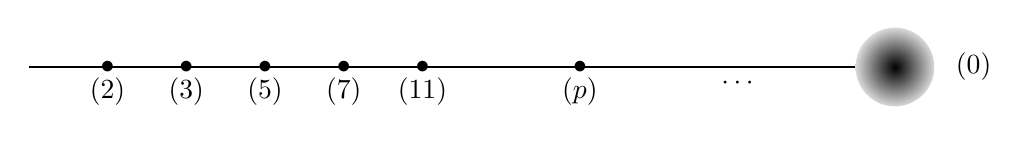
\begin{tikzpicture}
% Non-zero primes (closed points)
\draw[thick] (0,0)
    -- (1,0) node {\(\bullet\)} node[below] {\((2)\)}
    -- (2,0) node {\(\bullet\)} node[below] {\((3)\)}
    -- (3,0) node {\(\bullet\)} node[below] {\((5)\)}
    -- (4,0) node {\(\bullet\)} node[below] {\((7)\)}
    -- (5,0) node {\(\bullet\)} node[below] {\((11)\)}
    -- (7,0) node {\(\bullet\)} node[below] {\((p)\)}
    -- (9,0) node[below] {\(\cdots\)}
    -- (11,0);
% Generic point
\shade[inner color=black, outer color=gray!30]
    (11,0) circle (0.5);
\draw (12,0) node {\((0)\)};
\end{tikzpicture}

\noindent
(ii) $\Spec(\mathbf R)$.
Since $\mathbf R$ is a field, its only prime ideal is $(0)$.
Therefore $\Spec(\mathbf R)$ consists of a single point.

\noindent
(iii) $\Spec(\mathbf C[x])$.
Since $\mathbf C[x]$ is a PID, its non-zero prime ideals are generated by monic irreducible polynomials.
Moreover, since $\mathbf C$ is algebraically closed, these are exactly polynomials $x - a$, where $a \in \mathbf C$.
Again, the zero ideal is a generic point.
Therefore, $\Spec(\mathbf C[x])$ can be visualized like the following line, where $a$ varies continuously over $\mathbf C$.
\begin{center}
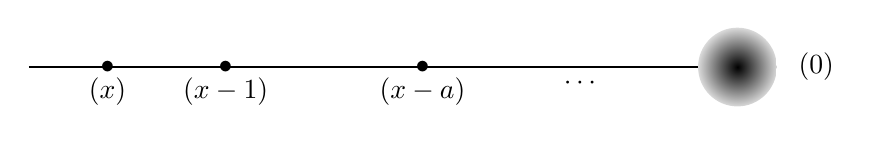
\begin{tikzpicture}

% Affine line
\draw[thick] (0,0)
    -- (1,0) node {$\bullet$} node[below] {$(x)$}
    -- (2.5,0) node {$\bullet$} node[below] {$(x-1)$}
    -- (5,0) node {$\bullet$} node[below] {$(x-a)$}
    -- (7,0) node[below] {$\cdots$}
    -- (9,0);


% Generic point
\shade[inner color=black, outer color=gray!30]
    (9,0) circle (0.5);
\draw (10,0) node {$(0)$};
\end{tikzpicture}
\end{center} 

\noindent
(iv) $\Spec(\mathbf R[x])$.
The non-zero prime ideals of $\mathbf R[x]$ correspond to monic irreducible polynomials over $\mathbf R$.
These are either of the form $x - a$ with $a \in \mathbf R$, or of the form $x^2 + bx + c$, with $b^2 - 4c < 0$.
Each polynomial of the latter type corresponds to two conjugate complex numbers (with non-zero imaginary part), the roots of the polynomial.
The zero ideal $(0)$ is a generic point.
Thus $\Spec(\mathbf R[x])$ can be seen as the complex plane folded along the real axis, with an extra generic point.
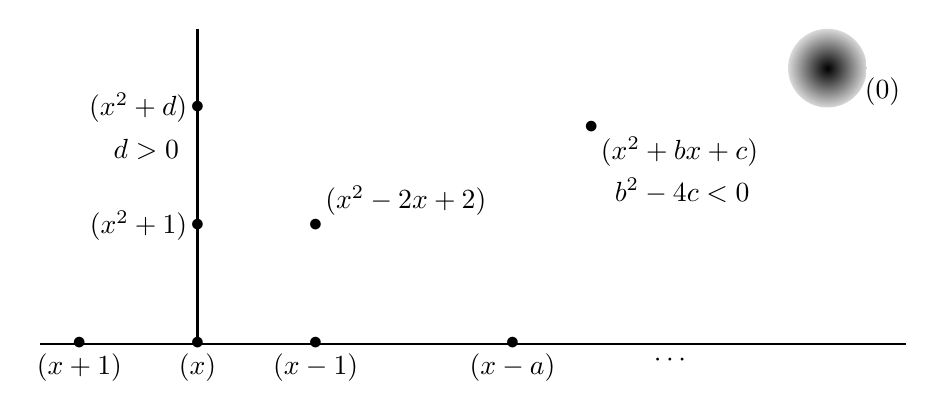
\begin{tikzpicture}
\draw[thick] (-1,0)
    -- (-0.5,0) node {$\bullet$} node[below] {$(x+1)$}
    -- (1,0) node {$\bullet$} node[below] {$(x)$}
    -- (2.5,0) node {$\bullet$} node[below] {$(x-1)$}
    -- (5,0) node {$\bullet$} node[below] {$(x-a)$}
    -- (7,0) node[below] {$\cdots$}
    -- (10,0);
\draw[thick] (1,0)
    -- (1,1.5) node {$\bullet$} node[left] {$(x^2 + 1)$}
    -- (1,3) node {$\bullet$} node[left] {$(x^2 + d)$} node[left, yshift=-15, xshift=-3] {$d > 0$}
    -- (1,4);
\draw (2.5,1.5) node {$\bullet$} node[above right] {$(x^2 - 2x + 2)$};
\draw (6,2.75) node {$\bullet$} node[below right] {$(x^2 + bx + c)$} node[below right, yshift=-15, xshift=5] {$b^2 - 4c < 0$};
\shade[inner color=black, outer color=gray!30] (9,3.5) circle (0.5);
\draw (9.7,3.2) node {$(0)$};
\end{tikzpicture}

\noindent
(v) $\Spec(\mathbf Z[x])$.
There is no better picture of $\Spec(\mathbf Z[x])$ than the following one, taken from \cite[II, \S1, Example H]{MumfordRedBook}.
\begin{center}
\includegraphics[width=0.9\textwidth]{atiyah-macdonald/images/Spec(Z[x])}
\end{center}














\begin{exercise}
\label{ex:1.17}
For each $f \in A$, let $X_f$, denote the complement of $V(f)$ in $X = \Spec(A)$.
The sets $X_f$, are open.
Show that they form a basis of open sets for the Zariski topology, and that
\begin{rlist}
\item
\label{ex:1.17.i}
$X_f \cap X_g = X_{f g}$;
\item
\label{ex:1.17.ii}
$X_f = \emptyset$ $\iff$ $f$ is nilpotent;
\item
\label{ex:1.17.iii}
$X_f = X$ $\iff$ $f$ is a unit;
\item
\label{ex:1.17.iv}
$X_f = X_g$ $\iff$ $r((f)) = r((g))$;
\item
\label{ex:1.17.v}
$X$ is quasi-compact (that is, every open covering of $X$ has a finite sub-covering).
\item
\label{ex:1.17.vi}
More generally, each $X_f$ is quasi-compact.
\item
\label{ex:1.17.vii}
An open subset of $X$ is quasi-compact if and only if it is a finite union of sets $X_f$.
\end{rlist}

The sets $X_f$ are called \emph{basic open sets} of $X = \Spec(A)$.

\noindent
[To prove \ref{ex:1.17.v}, remark that it is enough to consider a covering of $X$ by basic open sets $X_{f_i}$, ($i \in I$).
Show that the $f_i$ generate the unit ideal and hence that there is an equation of the form
\begin{equation*}
1 = \sum_{i \in J} g_i f_i
\qquad (g_i \in A)
\end{equation*}
where $J$ is some \emph{finite} subset of $I$.
Then the $X_{f_i}$ ($i \in J$) cover $X$.]
\end{exercise}

\begin{proof}
Let $U$ be an open set of $X$, and let $\mathfrak p \in U$ be given.
There is an ideal $\mathfrak a$ of $A$ such that $U$ is the complement of $V(\mathfrak a)$, so $\mathfrak a \not\subseteq \mathfrak p$.
Pick $f\in\mathfrak a$ such that $f\notin\mathfrak p$.
Thus $V(\mathfrak a) \subseteq V(f)$ and $\mathfrak p \in X_f$, so that $\mathfrak p \in X_f \subseteq U$.
This shows that the sets $X_f$ form a basis of open sets for the Zariski topology of $X$.
\end{proof}

\noindent
\ref{ex:1.17.i}
By Exercise \ref{ex:1.15}\ref{ex:1.15.iv}, we have $V(f g) = V(f) \cup V(g)$.
Taking complements gives $X_f \cap X_g = X_{f g}$.
\qed

\noindent
\ref{ex:1.17.ii}
$X_f = \emptyset$ $\iff$ $V(f) = X$ $\iff$ $f\in\mathfrak p$ for every prime ideal $\mathfrak p$ $\iff$ $f$ is nilpotent by Proposition 1.8.
\qed

\noindent
\ref{ex:1.17.iii}
$X_f = X$ $\iff$ $V(f) = \emptyset$ $\iff$ $f$ is not contained in any prime ideal $\iff$ $f$ is a unit by Corollary 1.5.
\qed

\noindent
\ref{ex:1.17.iv}
($\Leftarrow$)
If $r((f)) = r((g))$, then $V(f) = V(r((f))) = V(r((g))) = V(g)$ by Exercise \ref{ex:1.15}\ref{ex:1.15.i}, so $X_f = X_g$.

($\Rightarrow$)
Suppose $X_f = X_g$, so that $V(f) = V(g)$.
Let $x \in r((f))$ be given.
Then $x$ is contained in every prime ideal $\mathfrak p$ that contains $f$ by Proposition 1.14.
Since $V(f) = V(g)$, this means that $x$ is contained in every prime ideal $\mathfrak p$ that contains $g$, and hence we have $x \in r((g))$, again by Proposition 1.14.
This proves that $r((f))\subseteq r((g))$, and by the same argument we get that $r((g)) \subseteq r((f))$.
Thus, $r((f)) = r((g))$.
\qed

\noindent
\ref{ex:1.17.v}
This is a special case of \ref{ex:1.17.vi} since $X = X_1$ by \ref{ex:1.17.iii}.

\noindent
\ref{ex:1.17.vi}
Let $f\in A$ be given, and let $(U_i)_{i\in I}$ be an open covering of $X_f$.
Since $X_f$ is an open subset of $X$, a subset of $X_f$ is open in the subspace topology on $X_f$ if and only if it is open in the Zariski topology on $X$.
Thus each $U_i$ is also open in $X$.
Since the sets $X_g$ with $g\in A$ form a basis for the Zariski topology on $X$, it suffices to consider the case $U_i = X_{f_i}$, for some $f_i \in A$ ($i \in I$).
Thus, we have $\bigcup_{i\in I} X_{f_i} = X_f$, so that $\bigcap_{i\in I} V(f_i) = V(f)$.
By Exercise \ref{ex:1.15}\ref{ex:1.15.iii}, we conclude that $V\left(\bigcup_{i\in I} (f_i)\right) = V(f)$.
Let $\mathfrak a$ be the ideal generated by all the $f_i$ ($i\in I$).
Then $V(\mathfrak a) = V(f)$ by Exercise \ref{ex:1.15}\ref{ex:1.15.i}.
This implies that $f$ is contained in every prime ideal of $A$ that contains $\mathfrak a$.
By Proposition 1.14, it follows that $f \in r(\mathfrak a)$, whence $f^n \in \mathfrak a$ for some $n > 0$.
Thus, there exists a finite subset $J \subseteq I$ and a $g_i \in A$ for every $i \in J$ such that $f^n = \sum_{i\in J} g_i f_i$.
Let $\mathfrak b$ be the ideal generated by the $f_i$ ($i\in J$).
Then $f \in r(\mathfrak b)$, so $V(r(\mathfrak b)) \subseteq V(f)$.
Moreover, since $\mathfrak b \subseteq \mathfrak a$, it follows that $V(f) = V(\mathfrak a) \subseteq V(\mathfrak b) = V(r(\mathfrak b))$ by Exercise \ref{ex:1.15}\ref{ex:1.15.i}.
Thus $V(f) = V(\mathfrak b)$, so that by Exercise \ref{ex:1.15}\ref{ex:1.15.i}, Exercise \ref{ex:1.15}\ref{ex:1.15.iii}, and Corollary 1.4 we have
\begin{equation*}
\bigcap_{i \in J} V(f_i)
= V\left(\bigcup_{i\in J} (f_i)\right)
= V(\mathfrak b)
= V(f).
\end{equation*}
Taking complements shows that the family $(X_{f_i})_{i\in J}$ is an open covering of $X_f$, and it is a finite sub-covering of $(X_{f_i})_{i\in I}$.
Therefore, $X_f$ is quasi-compact.
\qed

\noindent
\ref{ex:1.17.vii}
Clearly a finite union of sets $X_f$ is both open and quasi-compact, since each $X_f$ is quasi-compact by \ref{ex:1.17.vi}.
Conversely, a quasi-compact subset $U$ of $X$ is covered by some family $(X_{f_i})_{i\in I}$, since the sets $X_f$ form a basis for the Zariski topology on $X$, and quasi-compactness implies that we can choose a finite sub-family of $(X_{f_i})_{i\in I}$ that still covers $U$.
\qed






\begin{exercise}
\label{ex:1.18}
For psychological reasons it is sometimes convinient to denote a prime ideal of $A$ by a letter such as $x$ or $y$ when thinking of it as a point of $X = \Spec(A)$.
When thinking of $x$ as a prime ideal of $A$, we denote it by $\mathfrak p_x$ (logically, of course, it is the same thing).
Show that
\begin{rlist}
\item
\label{ex:1.18.i}
the set $\{x\}$ is closed (we say that $x$ is a ``closed point'') in $\Spec(A)$ $\iff$ $\mathfrak p_x$ is maximal;
\item
\label{ex:1.18.ii}
$\overline{\{x\}} = V(\mathfrak p_x)$;
\item
\label{ex:1.18.iii}
$y \in \overline{\{x\}}$ $\iff$ $\mathfrak p_x \subseteq \mathfrak p_y$;
\item
\label{ex:1.18.iv}
$X$ is a $T_0$-space (this means that if $x,y$ are distinct points of $X$, then either there is a neighborhood of $x$ which does not contains $y$, or else there is a neighborhood of $y$ which does not contain $x$).
\end{rlist}
\end{exercise}

\noindent
\ref{ex:1.18.i}
($\Rightarrow$)
If $x$ is a closed point of $X$, then the only prime ideal containing $\mathfrak p_x$ is $\mathfrak p_x$ itself.
Since every ideal of $A$ other than $(1)$ is contained in a maximal ideal (Corollary 1.4), it follows that $\mathfrak p_x$ is maximal.

($\Leftarrow$)
If $\mathfrak p_x$ is maximal, than no other prime ideal of $A$ contains it, so $\{x\} = V(\mathfrak p_x)$.
Thus, $x$ is a closed point.
\qed

\noindent
\ref{ex:1.18.ii}
Since $\{x\} \subseteq V(\mathfrak p_x)$ and $V(\mathfrak p_x)$ is closed, it follows that $\overline{\{x\}} \subseteq V(\mathfrak p_x)$.
Next, let $E$ be a subset of $A$ such that $\overline{\{x\}} = V(E)$.
In paticular, $E \subseteq \mathfrak p_x$.
If $y \in V(\mathfrak p_x)$, then $\mathfrak p_x \subseteq \mathfrak p_y$, so $E \subseteq \mathfrak p_y$.
Thus, $y \in V(E) = \overline{\{x\}}$, and so $V(\mathfrak p_x) \subseteq \overline{\{x\}}$.
Therefore, $\overline{\{x\}} = V(\mathfrak p_x)$.
\qed

\noindent
\ref{ex:1.18.iii}
($\Rightarrow$)
Suppose $y \in \overline{\{x\}}$.
By \ref{ex:1.18.ii}, $\overline{\{x\}} = V(\mathfrak p_x)$, so $\mathfrak p_x \subseteq \mathfrak p_y$.

($\Leftarrow$)
Suppose $\mathfrak p_x \subseteq \mathfrak p_y$.
Then $y \in V(\mathfrak p_x) = \overline{\{x\}}$ by \ref{ex:1.18.ii}.
\qed

\noindent
\ref{ex:1.18.iv}
Let $x,y$ be distinct points of $X$.
Without loss of generality, assume $\mathfrak p_x \not\subseteq \mathfrak p_y$.
By \ref{ex:1.18.iii}, $y \notin \overline{\{x\}}$.
Then $X\setminus\overline{\{x\}}$ is a neighborhood of $y$ which does not contain $x$.
Thus, $X$ is a $T_0$-space.
\qed







\begin{exercise}
\label{ex:1.19}
A topological space $X$ is said to be irreducible if $X \neq \emptyset$ and if every pair of non-empty open sets in $X$ intersect, or equivalently if every non-empty open set is dense in $X$.
Show that $\Spec(A)$ is irreducible if and only if the nilradical of $A$ is a prime ideal.
\end{exercise}

\begin{proof}
Let $\mathfrak N$ denote the nilradical of $A$.

($\Rightarrow$)
Suppose $X=\Spec(A)$ is irreducible, and let $f,g\in A$ be given such that $f, g \notin \mathfrak N$.
By Exercise \ref{ex:1.17}\ref{ex:1.17.ii}, both $X_f$ and $X_g$ are nonempty open subsets of $X$.
By Exercise \ref{ex:1.17}\ref{ex:1.17.i}, $X_f \cap X_g = X_{f g}$, and since $X$ is irreducible, $X_f \cap X_g \neq \emptyset$.
Thus $f g$ is not nilpotent by Exercise \ref{ex:1.17}\ref{ex:1.17.ii}, so $\mathfrak N$ is a prime ideal.

($\Leftarrow$)
Suppose $\mathfrak N$ is a prime ideal, and let $U,V$ be non-empty open subsets of $X$.
Pick points $x\in U$ and $y \in V$.
By Exercise \ref{ex:1.17}, there exist $f,g\in A$ such that $x \in X_f \subseteq U$ and $y \in X_g \subseteq V$.
Since $X_f$ and $X_g$ are nonempty, $f$ and $g$ are non nilpotent (Exercise \ref{ex:1.17}\ref{ex:1.17.ii}).
Since $\mathfrak N$ is a prime ideal, $f g$ is also non nilpotent, so $X_{f g} = X_f \cap X_g$ is nonempty (Exercise \ref{ex:1.17}\ref{ex:1.17.i}).
Since $X_f \cap X_g \subseteq U \cap V$, $U \cap V$ is nonempty, and so $X$ is irreducible.
\end{proof}







\begin{exercise}
\label{ex:1.20}
Let $X$ be a topological space.
\begin{rlist}
\item
\label{ex:1.20.i}
If $Y$ is an irreducible (Exercise \ref{ex:1.19}) subspace of $X$, then the closure $\overline Y$ of $Y$ in $X$ is irreducible.
\item
\label{ex:1.20.ii}
Every irreducible subspace of $X$ is contained in a maximal irreducible subspace.
\item
\label{ex:1.20.iii}
The maximal irreducible subspaces of $X$ are closed and cover $X$.
They are called the \emph{irreducible components} of $X$.
What are the irreducible components of a Hausdorff space?
\item
\label{ex:1.20.iv}
If $A$ is a ring and $X = \Spec(A)$, then the irreducible components of $X$ are the closed sets $V(\mathfrak p)$, where $\mathfrak p$ is a minimal prime ideal of $A$ (Exercise \ref{ex:1.8}).
\end{rlist}
\end{exercise}

\begin{claim}
\label{claim:1.20.irred}
A nonempty topological space $X$ is irreducible if and only if there are no proper closed subsets $X_1,X_2\subseteq X$ such that $X = X_1 \cup X_2$.
\end{claim}

\begin{proof}
($\Rightarrow$)
Suppose there are proper closed subsets $X_1,X_2\subseteq X$ such that $X_1 \cup X_2 = X$.
Then the open sets $X\setminus X_1$ and $X\setminus X_2$ are nonempty and do not intersect, so $X$ is not irreducible.

($\Leftarrow$)
Suppose there are no two proper closed subsets of $X$ whose union is $X$.
Let $U$ and $V$ be two nonempty open subsets of $X$.
If $U\cap V = \emptyset$, then $X = (X\setminus U) \cup (X\setminus V)$, a union of two proper closed subsets.
This is a contradiction, so $U\cap V \neq \emptyset$, and hence $X$ is irreducible.
\end{proof}

\noindent
\ref{ex:1.20.i}
Let $Y$ be an irreducible subspace of $X$, and suppose $\overline Y = Y_1 \cap Y_2$ with $Y_1$ and $Y_2$ closed subsets of $Y$.
Since $\overline Y$ is closed in $X$, so are $Y_1$ and $Y_2$.
Then $Y = (Y \cap Y_1) \cup (Y \cap Y_2)$, a union of closed subsets of $Y$.
Since $Y$ is irreducible, Claim \ref{claim:1.20.irred} implies that either $Y\cap Y_1 = Y$ or $Y \cap Y_2 = Y$.
Thus, either $Y \subseteq Y_1$ or $Y \subseteq Y_2$, and so either $\overline Y = Y_1$ or $\overline Y = Y_2$.
Therefore, $\overline Y$ is not a union of two proper closed sets, so by Claim \ref{claim:1.20.irred} $\overline Y$ is irreducible.
\qed

\noindent
\ref{ex:1.20.ii}
Let $Y$ be an irreducible subspace of $X$, and let $\Sigma$ be the set of all irreducible subspaces of $X$ containing $Y$, partially ordered by inclusion.
Let $C$ be a chain in $\Sigma$, and let $Y^\prime = \bigcup_{Z\in C} Z$.
Suppose $Y^\prime = Y_1 \cup Y_2$ for some proper closed subsets $Y_1$ and $Y_2$ of $Y^\prime$.
Then there exist $Z_1,Z_2\in C$ such that $Y_1\cap Z_1$ is a proper closed subset of $Z_1$ and $Y_2 \cap Z_2$ is a proper closed subset of $Z_2$.
Without loss of generality, assume $Z_1 \subseteq Z_2$.
Then $Y_1 \cap Z_2$ is a proper closed subset of $Z_2$, and we have $Z_2 = (Y_1 \cap Z_2) \cup (Y_2 \cap Z_2)$, a contradiction by Claim \ref{claim:1.20.irred} since $Z_2$ is irreducible.
Thus, $Y^\prime$ is not a union of two proper closed subsets, so it is irreducible.
Hence $C$ has an upper bound in $\Sigma$, and so $\Sigma$ has maximal elements by Zorn's lemma.
That is, $Y$ is contained in a maximal irreducible subspace.
\qed

\noindent
\ref{ex:1.20.iii}
Let $Y$ be a maximal irreducible subspace of $X$.
By \ref{ex:1.20.i}, $\overline Y$ is also irreducible and $Y \subseteq \overline Y$, so $Y = \overline Y$ by the maximality of $Y$.
Therefore, maximal irreducible subspaces of $X$ are closed.
Next, let $x\in X$ be given.
The singleton $\{x\}$ is an irreducible subspace of $X$, so it is contained in some maximal irreducible subspace of $X$ by \ref{ex:1.20.ii}.
Thus, maximal irreducible subsets cover $X$.

If $X$ is a Hausdorff space, then its irreducible components are the sets $\{x\}$ for $x \in X$.
This is because in every subset of $X$ with at least two points, these points could be separated by open sets (by the Hausdorff condition), and so the subset is not irreducible.
\qed

\noindent
\ref{ex:1.20.iv}
This follows immediately from the following claim.

\begin{claim}
\label{claim:1.20.prime}
Let $A$ be a commutative ring.
The assignment $\mathfrak p \mapsto V(\mathfrak p)$ is an inclusion-reversing bijection between $X=\Spec(A)$ and its closed irreducible subspaces.
\end{claim}

\begin{proof}
Let $\mathfrak p$ be a prime ideal of $A$.
Suppose $V(\mathfrak p)$ can be written as the union of two proper closed subsets $Y,Z\subseteq V(\mathfrak p)$.
Since $V(\mathfrak p)$ is closed in $X$, both $Y$ and $Z$ are closed in $X$ as well, and hence there exist ideals $\mathfrak a,\mathfrak b$ of $A$ such that $Y=V(\mathfrak a)$ and $Z = V(\mathfrak b)$.
Thus, we have $V(\mathfrak a) \subseteq V(\mathfrak p)$, $V(\mathfrak b) \subseteq V(\mathfrak p)$, and $V(\mathfrak p) = V(\mathfrak a) \cup V(\mathfrak b)$.
By Exercise \ref{ex:1.15}\ref{ex:1.15.iv}, we have $V(\mathfrak p) = V(\mathfrak a) \cup V(\mathfrak b) = V(\mathfrak a \mathfrak b)$.
In particular, $\mathfrak a\mathfrak b \subseteq \mathfrak p$.
Then either $\mathfrak a \subseteq \mathfrak p$ or $\mathfrak b \subseteq \mathfrak p$ (otherwise, there exist $x\in \mathfrak a\setminus\mathfrak p$ and $y\in \mathfrak b\setminus \mathfrak p$ such that $x y \in \mathfrak a \mathfrak b \subseteq \mathfrak p$, a contradiction).
It follows that either $V(\mathfrak p)\subseteq V(\mathfrak a)$ or $V(\mathfrak p)\subseteq V(\mathfrak b)$, and hence either $V(\mathfrak p) = V(\mathfrak a)$ or $V(\mathfrak p) = V(\mathfrak b)$.
Hence $V(\mathfrak p)$ cannot be written as a union of two proper closed subsets, so $V(\mathfrak p)$ is irreducible by Claim \ref{claim:1.20.irred}.

Therefore, the assignment $\mathfrak p \mapsto V(\mathfrak p)$ sends prime ideals of $A$ to closed irreducible subsets of $X$, and it is clear that if $\mathfrak p,\mathfrak q\in \Spec(A)$ with $\mathfrak p \subseteq \mathfrak q$, then $V(\mathfrak q) \subseteq V(\mathfrak p)$.
Conversely, if $V(\mathfrak q) \subseteq V(\mathfrak p)$, then $\mathfrak q \in V(\mathfrak p)$, so $\mathfrak p \subseteq \mathfrak q$.
Thus, the assignment $\mathfrak p \mapsto V(\mathfrak p)$ is inclusion-reversing and injective.

Finally, we claim that every closed irreducible subspace of $X$ is of the form $V(\mathfrak p)$ for some prime ideal $\mathfrak p$ of $A$.
Let $V(\mathfrak a)$ be a closed irreducible subspace of $X$, for some ideal $\mathfrak a$ of $A$.
By Exercise \ref{ex:1.15}\ref{ex:1.15.i}, we may assume without loss of generality that $\mathfrak a = r(\mathfrak a)$.
Suppose $x, y \in A$ such that $x y\in \mathfrak a$.
It follows that $V(\mathfrak a) \subseteq V(x y) = V(x) \cup V(y)$ by Exercise \ref{ex:1.15}\ref{ex:1.15.iv}.
Since $V(\mathfrak a)$ is irreducible, Claim \ref{claim:1.20.irred} implies that either $V(\mathfrak a) = V(\mathfrak a)\cap V(x)$ or $V(\mathfrak a) = V(\mathfrak a)\cap V(y)$.
Without loss of generality, assume that $V(\mathfrak a) = V(\mathfrak a) \cap V(x)$.
It follows that $V(\mathfrak a) \subseteq V(x)$, so for every prime ideal $\mathfrak p$ of $A$ containing $\mathfrak a$, we have $x \in \mathfrak p$.
Since $\mathfrak a = r(\mathfrak a)$, Proposition 1.14 implies that $\mathfrak a$ is the intersection of all the prime ideals of $A$ containing $\mathfrak a$.
Thus, since $x\in\mathfrak p$ for all $\mathfrak p\in V(\mathfrak a)$, it follows that $x \in \mathfrak a$, and so $\mathfrak a$ is a prime ideal.
\end{proof}




\begin{exercise}
\label{ex:1.21}
Let $\phi : A \to B$ be a ring homomorphism.
Let $X = \Spec(A)$ and $Y = \Spec(B)$.
If $\mathfrak p \in Y$, then $\phi^{-1}(\mathfrak q)$ is a prime ideal of $A$, i.e., a point of $X$.
Hence $\phi$ induces a mapping $\phi^* : Y \to X$.
Show that
\begin{rlist}
\item
\label{ex:1.21.i}
If $f \in A$ then ${\phi^*}^{-1}(X_f) = Y_{\phi(f)}$, and hence that $\phi^*$ is continuous.
\item
\label{ex:1.21.ii}
If $\mathfrak a$ is an ideal of $A$, then ${\phi^*}^{-1}(V(\mathfrak a)) = V(\mathfrak a^e)$.
\item
\label{ex:1.21.iii}
If $\mathfrak b$ is an ideal of $B$, then $\overline{\phi^*(V(\mathfrak b))} = V(\mathfrak b^c)$.
\item
\label{ex:1.21.iv}
If $\phi$ is surjective, then $\phi^*$ is a homeomorphism of $Y$ onto the closed subset $V(\Ker(\phi))$ of $X$.
(In particular, $\Spec(A)$ and $\Spec(A/\mathfrak N)$ (where $\mathfrak N$ is the nilradical of $A$) are naturally homeomorphic.)
\item
\label{ex:1.21.v}
If $\phi$ is injective, then $\phi^*(Y)$ is dense in $X$.
More precisely, $\phi^*(Y)$ is dense in $X$ $\iff$ $\Ker(\phi) \subseteq \mathfrak N$.
\item
\label{ex:1.21.vi}
Let $\psi : B \to C$ be another ring homomorphism.
Then $(\psi \circ \phi)^* = \phi^* \circ \psi^*$.
\item
\label{ex:1.21.vii}
Let $A$ be an integral domain with just one non-zero prime ideal $\mathfrak p$, and let $K$ be the field of fractions of $A$.
Let $B = (A/\mathfrak p)\times K$.
Define $\phi : A \to B$ by $\phi(x) = (\overline x,x)$, where $\overline x$ is the image of $x$ in $A/\mathfrak p$.
Show that $\phi^*$ is bijective but not a homeomorphism.
\end{rlist}
\end{exercise}

\noindent
\ref{ex:1.21.i}
For a prime ideal $\mathfrak q$ of $B$ and an element $f \in A$, we have $\mathfrak q \in {\phi^*}^{-1}(X_f)$ if and only if $\phi^*(\mathfrak q) \in X_f$.
The latter is equivalent to $f \notin \phi^*(\mathfrak q)$, which is true if and only if $\phi(f) \notin \mathfrak q$ (i.e., if $\mathfrak q \in Y_{\phi(f)}$).
These equivalences imply that ${\phi^*}^{-1}(X_f) = Y_{\phi(f)}$.
Moreover, since the sets $X_f$ form a basis of open sets of $X$ (by Exercise \ref{ex:1.15}), it follows that the preimages of open subsets of $Y$ under $\phi^*$ are open subsets of $X$, whence $\phi^*$ is continuous.
\qed

\noindent
\ref{ex:1.21.ii}
Let $\mathfrak a$ be an ideal of $A$, and let $\mathfrak q$ be a prime ideal of $B$.
Then $\mathfrak q \in {\phi^*}^{-1}(V(\mathfrak a))$ if and only if $\phi^*(\mathfrak q) \in V(\mathfrak a)$, which holds if and only if $\mathfrak a \subseteq \phi^*(\mathfrak q)$.
The latter holds if and only if $\phi(\mathfrak a) \subseteq \mathfrak q$, which is equivalent to $\mathfrak q \in V(\phi(\mathfrak a)) = V(\mathfrak a^e)$ (the equality here is by Exercise \ref{ex:1.15}\ref{ex:1.15.i}).
Thus, ${\phi^*}^{-1}(V(\mathfrak a)) = V(\mathfrak a^e)$.
(Note that this also proves that $\phi^*$ is continuous since preimages of closed sets are closed.)
\qed


\noindent
\ref{ex:1.21.iii}
Let $\mathfrak b$ be an ideal of $B$, and let $\mathfrak p \in \phi^*(V(\mathfrak b))$.
Then there exists a $\mathfrak q \in V(\mathfrak b)$ such that $\mathfrak p = \phi^*(\mathfrak q)$.
That is, $\mathfrak b \subseteq \mathfrak q$, and therefore $\mathfrak b^c = \phi^{-1}(\mathfrak b) \subseteq \phi^*(\mathfrak q) = \mathfrak p$.
Thus $\mathfrak p \in V(\mathfrak b^c)$, and so $\phi^*(V(\mathfrak b)) \subseteq V(\mathfrak b^c)$.
Since $V(\mathfrak b^c)$ is closed, it follows that $\overline{\phi^*(V(\mathfrak b))} \subseteq V(\mathfrak b^c)$.

Next, let $U = X \setminus \overline{\phi^*(V(\mathfrak b))}$, and take $\mathfrak p \in U$.
Since $U$ is open, there exists an $f \in A$ such that $\mathfrak p \in X_f \subseteq U$.
That is, $f \notin \mathfrak p$ and, in particular, $X_f \subseteq X\setminus \phi^*(V(\mathfrak b))$.
This inclusion implies that $\phi^*(V(\mathfrak b)) \subseteq V((f))$.
Thus, for $\mathfrak q \in V(\mathfrak b)$, we have $f \in \phi^*(\mathfrak q)$ (i.e., $\phi(f) \in \mathfrak q$).
It follows that $\phi(f) \in \bigcap_{\mathfrak q \in V(\mathfrak b)} \mathfrak q$, so by Proposition 1.14, $\phi(f) \in r(\mathfrak b)$.
We then have $f \in \phi^{-1}(r(\mathfrak b)) = r(\mathfrak b)^c$, which implies, since $f \notin \mathfrak p$, that $r(\mathfrak b)^c \not\subseteq \mathfrak p$.
Thus, since $r(\mathfrak b)^c = r(\mathfrak b^c)$, we have $\mathfrak p \notin V(r(\mathfrak b^c)) = V(\mathfrak b^c)$ by Exercise \ref{ex:1.15}\ref{ex:1.15.i}.
Therefore, $U = X \setminus \overline{\phi^*(V(\mathfrak b))} \subseteq X\setminus V(\mathfrak b^c)$.
Taking complements, we see that $V(\mathfrak b^c) \subseteq \overline{\phi^*(V(\mathfrak b))}$, and so these two sets are equal.
\qed

\noindent
\ref{ex:1.21.iv}
Suppose $\phi$ is surjective.
Then $B \cong A/\Ker(\phi)$.
It is clear that, in this case, $\Spec(B)$ and $\Spec(A/\Ker(\varphi))$ are homeomorphic, so we can assume, without loss of generality, that $B = A/\mathfrak a$ for some ideal $\mathfrak a$ of $A$, and that $\phi : A \to A/\mathfrak a$ is the canonical projection map.
We must therefore prove that $Y = \Spec(A/\mathfrak a)$ is homeomorphic to $V(\mathfrak a)$ via $\phi^*$.

By Proposition 1.1, $\phi^*(Y) = V(\mathfrak a)$ and $\phi^*$ is injective, so $\phi^*$ is a continuous (by \ref{ex:1.21.i}) bijection onto the closed subset $V(\mathfrak a)$ of $X$.
Thus, to prove that $\phi^*$ is a homeomorphism, it suffices to prove that $\phi^*$ is a closed map.
Let $Y^\prime$ be a closed subset of $Y$, and let $\mathfrak b$ be an ideal of $B$ such that $Y^\prime = V(\mathfrak b)$.
By \ref{ex:1.21.iii}, we have $\overline{\phi^*(V(\mathfrak b))} = V(\mathfrak b^c)$, so in particular, $\phi^*(V(\mathfrak b)) \subseteq V(\mathfrak b^c)$.
Next, suppose $\mathfrak p \in V(\mathfrak b^c)$, and let $\mathfrak q$ be the prime ideal of $B$ such that $\mathfrak p = \phi^*(\mathfrak q)$.
Then $\mathfrak b^c \subseteq \mathfrak p$, so that $\mathfrak b \subseteq \mathfrak q$.
Then $\mathfrak q \in V(\mathfrak b)$, so that $\mathfrak p \in \phi^*(V(\mathfrak b))$.
This shows that $V(\mathfrak b^c) \subseteq \phi^*(V(\mathfrak b))$, so that these two sets are equal, and hence $\phi^*$ maps closed sets to closed sets.
Thus, $\phi^*$ is a homeomorphism of $Y$ onto $V(\mathfrak a)$.

If $\mathfrak a = \mathfrak N$, then $V(\mathfrak a) = X$ since $\mathfrak N$ is the intersection of all the prime ideals of $A$ by Proposition 1.8.
Thus, $X=\Spec(A)$ is homeomorphic to $\Spec(A/\mathfrak N)$.
\qed

\noindent
\ref{ex:1.21.v}
Note that
\begin{equation*}
V(\Ker(\phi))
= V((0)^c)
= \overline{\phi^*(V(0))}
= \overline{\phi^*(Y)},
\end{equation*}
where the middle equality is by \ref{ex:1.21.iii} and the last one is by Exercise \ref{ex:1.15}\ref{ex:1.15.ii}.
Thus, $\phi^*(Y)$ is dense in $X$ if and only if
\begin{equation*}
X
= \overline{\phi^*(Y)}
= V(\Ker(\phi)).
\end{equation*}
This is true if and only if $\Ker(\phi)$ is contained in every prime ideal of $A$, i.e., if and only if $\Ker(\phi) \subseteq \mathfrak N$ by Proposition 1.8.
Thus, $\phi^*(Y)$ is dense in $X$ if and only if $\Ker(\phi) \subseteq \mathfrak N$.

In particular, if $\phi$ is injective, then $\Ker(\phi) = (0) \subseteq \mathfrak N$, so $\phi^*(Y)$ is dense in $X$.
\qed

\noindent
\ref{ex:1.21.vi}
This is clear.
\qed

\noindent
\ref{ex:1.21.vii}
Let $A$ be an integral domain with exactly one non-zero prime ideal $\mathfrak p$, and let $K$ be the field of fractions of $A$.
Let $B = (A/\mathfrak p) \times K$, and let $\phi : A \to B$ be the ring homomorphism given by $\phi(x) = (\overline x, x)$, where $\overline x$ is the image of $x\in A$ in $A/\mathfrak p$.
Let $X = \Spec(A)$ and $Y = \Spec(B)$, and let $\phi* : Y \to X$ be the induced continuous map.
Then $X = \{0,\mathfrak p\}$.
Moreover, it is clear that the only prime ideals of $B$, both of which are maximal, are $(A/\mathfrak p) \times (0)$, whose image under $\phi^*$ is $(0)$, and $(0) \times K$, whose image under $\phi^*$ is $\mathfrak p$.
Thus, $\phi^*$ is bijective.
However, the point $(A/\mathfrak p) \times (0)$ of $Y$ is closed (by Exercise \ref{ex:1.18}\ref{ex:1.18.i}), but its image $(0)$ is not closed in $X$ since $(0)$ is not maximal.
Thus, there is a closed subset of $Y$ whose image under $\phi^*$ is not closed, so $\phi^*$ is not a homeomorphism.
\qed










\begin{exercise}
\label{ex:1.22}
Let $A = \prod_{i=1}^n A_i$ be the direct product of rings $A_i$.
Show that $\Spec(A)$ is the disjoint union of open (and closed) subspaces $X_i$, where $X_i$ is canonically homeomorphic with $\Spec(A_i)$.

Conversely, let $A$ be any ring.
Show that the following statements are equivalent:
\begin{rlist}
\item
\label{ex:1.22.i}
$X = \Spec(A)$ is disconnected.
\item
\label{ex:1.22.ii}
$A \cong A_1 \times A_2$ where neither of the rings $A_1,A_2$ is the zero ring.
\item
\label{ex:1.22.iii}
$A$ contains an idempotent $\neq 0,1$.
\end{rlist}

In particular, the spectrum of a local ring is always connected (Exercise \ref{ex:1.12}).
\end{exercise}

\begin{proof}



\end{proof}











\newpage







\begin{exercise}
\label{ex:1.23}
Let $A$ be a Boolean ring (Exercise \ref{ex:1.11}), and let $X = \Spec(A)$.
\begin{rlist}
\item
\label{ex:1.23.i}
For each $f \in A$, the set $X_f$ (Exercise \ref{ex:1.17}) is both open and closed in $X$.
\item
\label{ex:1.23.ii}
Let $f_1,\ldots,f_n \in A$.
Show that $X_{f_1} \cup \cdots \cup X_{f_n} = X_f$ for some $f \in A$.
\item
\label{ex:1.23.iii}
The sets $X_f$ are the only subsets of $X$ which are both open and closed.
[Let $Y \subseteq X$ be both open and closed.
Since $Y$ is open, it is a union of basic open sets $X_f$.
Since $Y$ is closed and $X$ is quasi-compact (Exercise \ref{ex:1.17}), $Y$ is quasi-compact.
Hence $Y$ is a finite union of basic open sets; now use \ref{ex:1.23.ii} above.]
\item
\label{ex:1.23.iv}
$X$ is a compact Hausdorff space.
\end{rlist}
\end{exercise}

\noindent
\ref{ex:1.23.i}
Let $f \in A$ be given.
Then $X_f$ is necessarily open since it is the complement in $X$ of the closed set $V((f))$.
We will prove that $X_f$ is also closed by proving that its complement $V((f))$ is open.
Suppose $\mathfrak p \in V((f))$, so that $f \in \mathfrak p$.
Let $g = 1 - f$.
Then $g \notin \mathfrak p$ (otherwise, $1 = f + g \in \mathfrak p$), so $\mathfrak p \in X_g$.
Now suppose $\mathfrak q \in X_g$.
Then $g \notin \mathfrak q$, so $g$ is $1$ modulo $\mathfrak q$ since $A/\mathfrak q$ is a field with two elements by Exercise \ref{ex:1.11}\ref{ex:1.11.ii}.
That is, $f = 1 - g \in \mathfrak q$, and so $\mathfrak q \in V((f))$.
Thus, we have $\mathfrak p \in X_g \subseteq V((f))$, so every point of $V((f))$ is contained in a basic open set contained in $V((f))$.
Therefore, $V((f))$ is open.
\qed

\noindent
\ref{ex:1.23.ii}
Let $f_1,\ldots,f_n \in A$, and let $\mathfrak a$ be the ideal in $A$ generated by $f_1,\ldots,f_n$.
From Exercise \ref{ex:1.11}\ref{ex:1.11.iii} it follows that $\mathfrak a = (f)$ for some $f \in A$.
Thus, for a prime ideal $\mathfrak p$ of $A$, we have $f \in \mathfrak p$ if and only if $f_1,\ldots,f_n \in \mathfrak p$.
Equivalently, $f \notin \mathfrak p$ if and only if $f_i \notin \mathfrak p$ for some $i\in\{1,\ldots,n\}$, and this implies that $X_f = X_{f_1}\cup \cdots \cup X_{f_n}$.
\qed

\noindent
\ref{ex:1.23.iii}
Let $Y \subseteq X$ be both open and closed.
Since $Y$ is closed and $X$ is quasi-compact (Exercise \ref{ex:1.17}\ref{ex:1.17.v}), $Y$ is quasi-compact (\emph{Proof.} any open cover of $Y$ can be extended to an open cover of $X$ by including the complement of $Y$, and only finitely many of the sets in this cover are required to cover $X$, whence only finitely many of the sets in the original cover are required to cover $Y$).
Since $Y$ is open and quasi-compact, $Y$ is a finite union of basic open sets by Exercise \ref{ex:1.17}\ref{ex:1.17.vii}.
Thus, $Y$ is equal to $X_f$ for some $f\in A$ by \ref{ex:1.23.ii}, and this, together with \ref{ex:1.23.i}, implies that the only open and closed subsets of $X$ are of the form $X_f$ with $f\in A$.
\qed

\noindent
\ref{ex:1.23.iv}
We know that $X$ is quasi-compact by Exercise \ref{ex:1.17}\ref{ex:1.17.v}, so it suffices to prove that $X$ is Hausdorff.
Let $\mathfrak p,\mathfrak q \in X$ be distinct points.
By Exercise \ref{ex:1.11}\ref{ex:1.11.ii}, both $\mathfrak p$ and $\mathfrak q$ are maximal ideals of $A$, so they must be coprime since they are distinct.
That is, $\mathfrak p + \mathfrak q = (1)$, so there exist $f\in\mathfrak p$ and $g \in \mathfrak q$ such that $f + g = 1$.
Then $f \notin \mathfrak q$ and $g \notin \mathfrak p$, so $X_f$ is an open neighborhood of $\mathfrak q$ which does not contain $\mathfrak p$, and $X_g$ is an open neighborhood of $\mathfrak p$ which does not contain $\mathfrak q$.
Therefore, $X$ is Hausdorff.
\qed



\begin{exercise}
\label{ex:1.24}
Let $L$ be a lattice, in which the $\sup$ and $\inf$ of two elements $a,b$ are denoted by $a \vee b$ and $a \wedge b$ respectively.
$L$ is a \emph{Boolean lattice} (or \emph{Boolean algebra}) if
\begin{rlist}
\item
\label{ex:1.24.i}
$L$ has a least element and a greatest element (denoted by $0,1$ respectively).
\item
\label{ex:1.24.ii}
Each of $\vee$, $\wedge$ is distributive over the other.
\item
\label{ex:1.24.iii}
Each $a \in L$ has a unique ``complement'' $a^\prime \in L$ such that $a \vee a^\prime = 1$ and $a \wedge a^\prime = 0$.
\end{rlist}
(For example, the set of all subsets of a set, ordered by inclusion, is a Boolean lattice.)

Let $L$ be a Boolean lattice.
Define addition and multiplication in $L$ by the rules
\begin{equation*}
a + b
= (a \wedge b^\prime) \vee (a^\prime \wedge b),
\qquad
a b
= a \wedge b.
\end{equation*}
Verify that in this way $L$ becomes a Boolean ring, say $A(L)$.

Conversely, starting from a Boolean ring $A$, define an ordering on $A$ as follows:
$a \leq b$ means that $a = a b$.
Show that, with respect to this ordering, $A$ is a Boolean lattice.
[The $\sup$ and $\inf$ are given by $a \vee b = a + b + a b$ and $a \wedge b = ab$, and the complement by $a^\prime = 1 - a$.]
In this way we obtain a one-to-one correspondence between (isomorphism classes of) Boolean rings and (isomorphism classes of) Boolean lattices.
\end{exercise}

\begin{proof}
Let $L$ be a Boolean lattice, and define addition and multiplication on $L$ as above.
Note that both $\vee$ and $\wedge$ are associative and commutative, so for $a,b\in L$, we have
\begin{align*}
(a \vee b) \wedge (a^\prime \wedge b^\prime)
&= (a \wedge a^\prime \wedge b^\prime) \vee (b \wedge a^\prime \wedge b^\prime)
\\&= (0 \wedge b^\prime) \vee (a^\prime \wedge b \wedge b^\prime)
\\&= 0 \vee (a^\prime \wedge 0)
= a^\prime \wedge 0
= 0,
\\(a \vee b) \vee (a^\prime \wedge b^\prime)
&= (a \vee b \vee a^\prime) \wedge (a \vee b \vee b^\prime)
\\&= (b \vee a \vee a^\prime) \wedge (a \vee 1)
\\&= (b \vee 1) \wedge 1
= b \vee 1
= 1.
\end{align*}
Therefore,
\begin{equation*}
(a \vee b)^\prime = a^\prime \wedge b^\prime
\end{equation*}
by the uniqueness of complements.
By a similar calculation, we have
\begin{equation*}
(a \wedge b)^\prime = a^\prime \vee b^\prime.
\end{equation*}
(The preceding two equations are just DeMorgan's laws.)


Since $\vee$ and $\wedge$ are commutative, so is addition and multiplication.
If $a \in L$, then
\begin{equation*}
a + 0
= (a \wedge 0') \vee (a^\prime \wedge 0)
= (a \wedge 1) \vee 0
= a \wedge 1
= a,
\end{equation*}
so $0$ is the identity for addition.
Moreover, $1$ is the identity for multiplication since $a \wedge 1 = a$.
Next, we have
\begin{equation*}
a + a
= (a \wedge a^\prime) \vee (a^\prime \wedge a)
= 0 \vee 0
= 0,
\end{equation*}
so $a$ is the additive inverse of $a$.
If $a,b,c\in L$, then
\begin{align*}
a + (b + c)
&= (a \wedge (b + c)^\prime) \vee (a^\prime \wedge (b + c))
\\&= (a \wedge ((b \wedge c^\prime) \vee (b^\prime \wedge c))^\prime) \vee (a^\prime \wedge ((b \wedge c^\prime) \vee (b^\prime \wedge c)))
\\&= (a \wedge ((b \wedge c^\prime)^\prime \wedge (b^\prime \wedge c)^\prime)) \vee (a^\prime \wedge ((b \wedge c^\prime) \vee (b^\prime \wedge c)))
\\&= (a \wedge ((b^\prime \vee c^{\prime\prime}) \wedge (b^{\prime\prime} \vee c^\prime))) \vee (a^\prime \wedge ((b \wedge c^\prime) \vee (b^\prime \wedge c)))
\\&= (a \wedge ((b^\prime \vee c) \wedge (b \vee c^\prime))) \vee (a^\prime \wedge ((b \wedge c^\prime) \vee (b^\prime \wedge c)))
\end{align*}



???????



???????



???????



???????



???????



(This exercise is proved by Stone in \cite[Theorem 2]{StoneRepresentationOfBooleanAlgebras}.)
\end{proof}








\begin{exercise}
\label{ex:1.25}
From the last two exercises deduce Stone's theorem, that every Boolean lattice is isomorphic to the lattice of open-and-closed subsets of some compact Hausdorff space.
\end{exercise}

\begin{proof}
Let $L$ be a Boolean lattice, and let $A = A(L)$ be the Boolean ring constructed from $L$ in Exercise \ref{ex:1.24}.
Let $X = \Spec(A)$.
Then $X$ is a compact Hausdorf space by Exercise \ref{ex:1.23}\ref{ex:1.23.iv}.
Let $S$ be the set of open-and-closed subsets of $X$.
By Exercise \ref{ex:1.23}\ref{ex:1.23.iii}, $S = \{X_f \mid f \in A(L)\}$.
Define $\phi : L \to S$ by $\phi(f) = X_f$.
Clearly $\phi$ is surjective.
Next, suppose $f,g\in L$ and $f \neq g$.



???????



???????



???????



???????



???????










\end{proof}








\begin{exercise}
\label{ex:1.26}
Let $A$ be a ring.
The subspace of $\Spec(A)$ consisting of the \emph{maximal} ideals of $A$, with the induced topology, is called the \emph{maximal spectrum} of $A$ and is denoted by $\Max(A)$.
For arbitrary commutative rings it does not have the nice functorial properties of $\Spec(A)$ (see Exercise \ref{ex:1.21}), because the inverse image of a maximal ideal under a ring homomorphism need not be maximal.

Let $X$ be a compact Hausdorff space and let $C(X)$ denote the ring of all real-valued continuous functions on $X$ (add and multiply functions by adding and multiplying their values).
For each $x\in X$, let $\mathfrak m_x$ be the set of all $f\in C(X)$ such that $f(x)=0$.
The ideal $\mathfrak m_x$ is maximal, because it is the kernel of the (surjective) homomorphism $C(X)\to\mathbf R$ which takes $f$ to $f(x)$.
If $\tilde X$ denotes $\Max(C(X))$, we have therefore defined a mapping $\mu:X\to\tilde X$, namely $x\mapsto\mathfrak m_x$.

We shall show that $\mu$ is a homeomorphism of $X$ onto $\tilde X$.
\begin{rlist}
\item\label{ex:1.26.i}
Let $\mathfrak m$ be any maximal ideal of $C(X)$, and let $V=V(\mathfrak m)$ be the set of common zeros of the functions in $\mathfrak m$: that is,
\begin{equation*}
V = \{x\in X : f(x) = 0 \text{ for all } f\in\mathfrak m\}.
\end{equation*}
Suppose that $V$ is empty.
Then for each $x\in X$ there exists $f_x\in\mathfrak m$ such that $f_x(x)\neq 0$.
Since $f_x$ is continuous, there is an open neighborhood $U_x$ of $x$ in $X$ on which $f_x$ does not vanish.
By compactness a finite number of the neighborhoods, say $U_{x_1},\ldots,U_{x_n}$, cover $X$.
Let
\[
f = f_{x_1}^2 + \cdots + f_{x_n}^2.
\]
Then $f$ does not vanish at any point of $X$, hence is a unit in $C(X)$.
But this contradicts $f\in\mathfrak m$, hence $V$ is not empty.

Let $x$ be a point of $V$.
Then $\mathfrak m \subseteq \mathfrak m_x$, hence $\mathfrak m = \mathfrak m_x$, since $\mathfrak m$ is maximal.
Hence $\mu$ is surjective.
\item\label{ex:1.26.ii}
By Urysohn's lemma (this is the only non-trivial fact required in the argument) the continuous functions separate the points of $X$.
Hence $x\neq y\implies\mathfrak m_x\neq \mathfrak m_y$, and therefore $\mu$ is injective.
\item\label{ex:1.26.iii}
Let $f\in C(X)$; let
\[
U_f = \{x\in X \mid f(x)\neq 0\}
\]
and let
\[
\tilde U_f = \{\mathfrak m\in\tilde X \mid f\notin\mathfrak m\}.
\]
Show that $\mu(U_f)=\tilde U_f$.
The open sets $U_f$ (resp. $\tilde U_f$) form a basis of the topology of $X$ (resp. $\tilde X$) and therefore $\mu$ is a homeomorphism.
Thus $X$ can be reconstructed from the ring of functions $C(X)$.
\end{rlist}
\end{exercise}

\noindent
\ref{ex:1.26.i}
Let $\mathfrak m$ be a maximal ideal of $C(X)$, and let $V=V(\mathfrak m) = \{x\in X : f(x) = 0 \text{ for all  } f\in\mathfrak m\}$.
Suppose $V=\emptyset$.
Then for each $x\in X$ there exists $f_x\in\mathfrak m$ such that $f_x(x)\neq 0$.
Since each $f_x$ is continuous, there is an open neighborhood $U_x$ of $x$ in $X$ such that $f_x(y)\neq 0$ for all $y\in U_x$.
Then the set $\{U_x\}_{x\in X}$ is an open cover of the compact space $X$, so there is a finite subcover $\{U_{x_i}\}_{i=1}^n$ of $X$.
Define
\[
f = f_{x_1}^2 + \cdots + f_{x_n}^2,
\]
and let $x\in X$ be given.
Then $x\in U_{x_i}$ for some $i\in\{1,\ldots,n\}$, so that $f_{x_i}(x)\neq 0$.
This implies that $f_{x_i}(x)^2 > 0$, and hence $f(x) > 0$.
Thus, $f(x)\neq 0$ for all $x\in X$, so $f$ is a unit in $C(X)$ (its inverse $g$ is the function $g(x)=1/f(x)$).
But since $f\in\mathfrak m$ and $\mathfrak m$ is a proper ideal of $C(X)$, $f$ cannot be a unit.
Thus, we have a contradiction, and hence $V$ is nonempty.
Let $x\in V$ be given.
Then we have $\mathfrak m \subseteq \mathfrak m_x$ for every $f\in\mathfrak m$ we have $f(x)=0$, and hence $f\in\mathfrak m_x$.
By the maximality of $\mathfrak m$, we conclude that $\mathfrak m = \mathfrak m_x$, and hence $\mathfrak m = \mu(x)$.
This shows that $\mu$ is surjective.
\qed

\noindent
\ref{ex:1.26.ii}
Let $x,y\in X$ be distinct points.
Because $X$ is Hausdorff and the sets $\{x\}$ and $\{y\}$ are compact, it follows that $\{x\}$ and $\{y\}$ are closed.
Since $X$ is Hausdorff and compact, it is normal (i.e., disjoint closed sets can be separated by open sets; cf. \cite[Chapter II, \S3, Theorem 3.5]{LangRealFunctionalAnalysis}), and hence by Urysohn's lemma (cf., e.g., \cite[Chapter II, \S4, Theorem 4.2]{LangRealFunctionalAnalysis}) there exists an $f\in C(X)$ such that $f(x)=0$ and $f(y)=1$.
Then $f\in\mathfrak m_x$, but $f\notin\mathfrak m_y$, so that $\mu(x)=\mathfrak m_x\neq \mathfrak m_y = \mu(y)$.
This shows that $\mu$ is injective.
\qed

\noindent
\ref{ex:1.26.iii}


?????

?????

?????

?????





\section*{Affine algebraic varieties}



\begin{exercise}
\label{ex:1.27}
\end{exercise}








\begin{exercise}
\label{ex:1.28}
\end{exercise}

































